\chapter{Úvod}\label{uvod}

Mestskú hromadnú opravu využíva takmer každý človek a preto sa oplatí pracovať na jej efektivite.
Zmyslom tejto práce je nazrieť do problematiky vytvárania a správy jednotlivých liniek mestksej hromadnej dopravy, ich analýze a optimalizácie, vytvoriť nástroj, ktorý pomôže analytikom pri vytváraní nových liniek alebo optimalizácii existujúcich.
Výsledkom celej práce je teoretické zefektívnenie mestskej hromadnej dopravy.

Mestská hromadná doprava je systém, ktorý je pre ľudí žijúcich v mestách a prímestských oblastiach existenčne dôležitý, preto sa oplatí investovať čas a námahu do jeho optimalizácie.
Kedže je problematika mestksej hromadnej dopravy aj mne blízka, z pohľadu cestujúceho sa s ňou stretávam každý deň, rozhodol som sa zamerať na túto tému.

Ľudia od nepamäti nachádzjú inšpiráciu pre takmer všetky svoje vynálezy v prírode a tomuto trendu neunikla ani informatika, ktorá má od prírody zo všetkých vedných oborov asi najďalej.
Algoritmy inšpirované prírodou prinášajú riešenia na problémy, ktoré by sme inými spôsobmi vedeli vyriešiť len za nereálne dlhý čas.
Táto časť informaiky ma veľmi zaujala a preto som sa rozhodol nájsť ďalšie možné využitie pre jeden z týchto algoritmov, ktoré sa používajú pre komplexné problémy s veľkým množstvom navzájom sa ovplyvňujúcich premenných.

Cieľom tejto práce je vytvoriť nástroj, ktorý za pomoci genetického algoritmu a používateľských obmedzení nájde optimálny časový rozpis jednej linky mestskej hromadnej dopravy.
Zároveň sa tento nástroj bude dať použiť na analýzu už existujúcich rozpisov.
Nástroj obsahuje uživateľské rozhranie pre rýchlu manipuláciu so vstupnými dátami a prehľadné zobrazenie výsledkov.
Použité technológie boli inšpírované prípadovou štúdiou~\cite{kate2021optimising}, ktorá pomocou simulácie a evolučných algoritmov dokázala optimalizovať cesty autonómnych vozidiel.

Práca je rozdelená na 7 kapitol vrátane úvodu a záveru, z toho najdoležitejšie sú kapitoly~\ref{relevantne_vlastnosti} až~\ref{nastroj}.

Na zostrojenie simulačného modelu je potrebné najprv získať informácie, vlastnosti reálneho systému a vyhodnotiť, ktoré z nich sú pre nás relevantné.
Kapitolo~\ref{relevantne_vlastnosti} popisuje konzultáciu s analytikom Dopravného podniku mesta Brno, ktorý popísal postupy a metódy, ktoré sa používajú pre optimalizáciu liniek v súčastnosti a vytýčil vlastnosti, na ktoré je dôležité sa zamerať pri simulácii a optimalizácii časového rozpisu linky.

Zo získaných informácií bol následne vytvorený simulačný model, ktorého popis je popísaný v kapitole~\ref{simulacny_model}.
Výstupy simulačného modelu sú základom pre optimalizáciu časového rozpisu linky.
Obsahujú sériu grafov, na ktorých používateľ vidí vyťaženosť linky v priebehu dňa a na jednotlivých zastávkach.
Získané výsledky boli použité k validácii simulačného modelu a na ohodnotenie jednotlivých rozpisov.

Kapitola~\ref{optimalizacia} popisuje proces optimalizácie časového rozpisu linky mestskej hromadnej dopravy.
Jednotlivé rozpisy ohodnotené na základe štatistík získaných zo simulácie budú použité ako jedinci v genetickom algoritme.
Genetický aloritmus následne tieto rozpisy kríži medzi sebou a mutuje, aby našiel čo optimálne riešenie.

Kapitola~\ref{experimenty} popisuje experimenty optimalizácie.
Aplikácia a optimalizačný algoritmus bol testovaný priebežne.
Kapitola obsahuje konkrétne experimenty, ktoré sa realizovali po dokončení vývoja,
skúmajúce správanie sa optimalizačného algoritmu vzhľadom na zmeny vstupov ako dĺžka trasy a kapacita vozidla.

Samotný algoritmus by nebol v praxi použiteľný bez používateľského rozhrania.
Kapitola~\ref{nastroj} popisuje návrh a implementácia uživateľského rozhrania analytického nástroja, umožňujúceho používateľovi jednoducho zadať vstupné dáta, spustiť analýzu a optimalizáciu časového rozpisu a vyhodnotiť výsledky.
Jednou z najdôležitejších častí tohto rozhrania je zadávanie používateľských obmedzení, ktoré musí výsledný časový rozpis obsahovať.

Záver~\ref{zaver} obsahuje zhrnutie dosiahnutých výsledkov tejto bakalárskej práce a možné budúce rozšírenia aplikácie.

\chapter{Relevantné vlastnosti mestskej hromadnej dopravy}\label{relevantne_vlastnosti}

Systém mestkej hromadnej dopravy je veľmi komplexný, obsahuje mnoho častí, na ktoré by bolo vhodné sa zamerať z pohľadu optimalizácie.
Prvým rozhodnutím je výber častí mestskej hromadnej dopravy, ktorá je vhodná na optimalizáciu.
Pre uskutočnenie správneho rozhodnutia sú potrebné informácie o reálnom systéme, doterajších postupoch, spôsoboch analýzy a optimalizácie.

\section{Konzultácia s analytikom Dopravného podniku}
Pre získanie relevantných informácií mi bolo doporučené obrátiť sa na pána Michaela Kříže, analytika Dopravného podniku mesta Brno (DPMB).
Stretnutie s pánom Křížom prebehlo 7. 10. 2024 v priestoroch administratívy DPMB.
Na základe získaných informácií som sa rozhodol zamerať na analýzu a optimalizáciu časového rozpisu jednej linky mestskej hromadnej dopravy.
Optimalizácia viac ako jednej linky naraz by pravdepodobne prinieslo lepšie výsledky, ale len v čisto teoretickej rovine.
V praxi je to z finančných a časových dôvodov neefektívne.
Vzájomne sme sa zhodli na tom, že najlepšie bude optimalizovať jednu linku a to iba jedným smerom, nakoľko druhý smer linky sa dá považovať za samostatnú linku, minimálne v rámci nárokov cestujúcej verejnosti.

\section{Získané relevantné vlastnosti}

Vlastnosti, ktoré sú potrebné pre správnu analýzu a optimalizáciu časového rozpisu linky mestskej hromadnej dopravy sú:

\begin{itemize}
  \item \textbf{Počet zastávok a informácie o nich} --- potrebné pre zostavenie samotného rozpisu aj simulačného modelu, nie je dôležitý len počet, ale aj informácie o jednotlivých zastávkach.
  \item \textbf{Čas jazdy medzi jednotlivými zastávkami} --- je to dôležitou súčasťou rozpisu, zároveň sa touto informáciou riadi plánovanie udalostí v simulačnom modeli, viac v kapitole~\ref{simulacny_model}.
  \item \textbf{Počet odchodov vozidla z jeho prvej zastávky za celý deň} --- celkový počet vozidiel, respektíve ciest, ktoré vozidlá danej linky za deň absolvujú. Tento parameter je dôležitý pre optimalizáciu, nakoľko pre dopravný podnik je výhodné mať čo najmenší počet vozidiel, ktoré vykonávajú obsluhu jednotlivých trás, šetrí to palivo, údržbu aj ľudské zdroje.
  \item \textbf{Počet odchodov vozidla z jeho prvej zastávky za hodinu} --- myslí sa tým jeden riadok časového rozpisu, mal by byť priamo úmerný priemernému počtu cestujúcich čakajúcich na danú linku v danej hodine.
  \item \textbf{Počet cestujúcich čakajúcich na jednotlivých zastávkach} --- časový rozpis by mal v čo najvyššej miere uspokojiť prepravné potreby väčšiny cestujúcich. Na prvotné testovacie účely boli použité hodnoty zodpovedajúce reálnemu počtu odchádzajúcich vozidiel za hodinu a ich kapacite dlhodobo existujúcej linky DPMB, ktorá je do veľej miery praxou optimalizovaná.
  \item \textbf{Doba čakania na zastávke} --- užitočný parameter pre analytika, ktorý slúži na overenie kvality časového rozpisu, ak je doba čakania na zastávke dlhá, je to známka toho, že rozpis nie je optimálny a je potrebné ho upraviť.
  \item \textbf{Počet cestujúcich vo vozidie} --- dôležitý parameter pre optimalizáciu. Vysoká preplnenosť vozidla má za dôsledok nekomfortné cestovanie, na druhej strane, príliš prázdne vozidlo je neefektívne pre dopravný podnik.
  \item \textbf{Kapacita vozidla} --- každé vozidlo má presne definovanú maximálnu kapacitu, zároveň sa od naplnenosti vozidla odvíja komfort cestujúcich. Informácie o kapacite konkrétných vozidiel sú získané z webovej stránky dopravného podniku~\cite{dpmb_vozy}.
  \item \textbf{Miest na sedenie} --- to či cestujúci sedí alebo bude musieť počas jazdy stáť ovplyvňuje jeho spokojnosť, ktorá výrazne ovplivňuje ohodnotenie rozpisu z pohľadu optimalizácie.
  \item \textbf{Počet cestujúcich, ktorí nenásúpia kvôli preplnenosti vozidla} --- v extrémnych prípadoch može nastať situácia, že bude vozidlo úplne plné a nebude možné aby do neho pristúpilo viac cestujúcich. Rozpisy, pri ktorých táto situácia vznikne budú veľmi negatívne ohodnocované z pohľadu optimalizácie aby sa táto nežiadúca situácia čo najviac eliminovala, viac v kapitole o optimalizácii~\ref{optimalizacia}.
  \item \textbf{Počet vystupujúcich cestujúcich na jednotlivých zastávkach} --- tento parameter je potrebný pre simuláciu, keďže do vozidla s presne definovanou kapacitou cestujúci priebežne nastupujú aj vystupujú. Každá zastávka má pridelený koeficient dôležitosti, ktorý určuje aký podiel z prepravovaných cestujúcich vystúpi na danej zastávke. Prvá zastávka má tento koeficient 0 (cestujúci iba nastupujú), na konečnej zastávke je koeficient 1 (cestujúci iba vystupujú). Na ostatných zastávkach sa koeficient mení podľa toho, aký podiel cestujúcich na danej zastávke priemerne vystupuje pričom prestupné zastávky majú vyšší koeficient ako neprestupné.
  \item \textbf{Náklady na prevádzku} --- náklady na prevádzku sú hlavným parametrom optimalizácie časových rozpisov jednotlivých liniek vyžadovaným DPMB. Náklady jednotlivých typov vozidiel sú súčasťou finančného plánu zahrnutého v zmluve~\cite{brno_dpmb_smlouva_2023}.
  \item \textbf{Dĺžka trasy} --- parameter potrebný na výpočet celkových nákladov na prevádzku linky. Dĺžky jednotlivých liniek sú obsahom zmluvy~\cite{brno_dpmb_smlouva_2023}.
\end{itemize}

\chapter{Simulačný model linky mestskej hromadnej dopravy}\label{simulacny_model}

Krokom následujúcim po získaní potrebných informácií je zostrojenie simulačného modelu.
Problém optimalizácie časového rozpisu linky mestskej hromadnej dopravy je veľmi komplexný.
Program, ktorý by tento problém riešil analytickým spôsobom by bol veľmi neefektívny a mal by priveľkú časovú zložitosť výpočtu.
Preto sme sa rozhodli využiť stochastický spôsob, to jest vytvorenie simulačného modelu, ktorého výstupy budú následne využité pri optimalizácii genetickým algoritmom.
Simulačný model bude reprezentovať jednu linku MHD, idúcu jedným smerom.
Časti modelu sú zastávky, vozidlá a cestujúci, pričom najdôležitejšou časťou je časový rozpis, ktorý obsahuje odchody jednotlivých vozidiel.
Na základe informácii získaných z priebehu simulácie sa rozpis ohodnotí a toto ohodnotenie sa využije v genetickom algoritme na jeho optimalizáciu.
Viac informácií o optimalizácii a genetickom algoritme je v kapitole~\ref{optimalizacia}.

\section{DEVS --- Discrete Event System Specification}
Na modelovanie bol použitý formalizmus DEVS (Discrete Event System Specification).
Všetky informácie o tomto formalizme v tejto sekcii sú čerpané zo zborníka z konferencie WSC 2018~\cite{tendeloo2018discrete}, kde je DEVS podrobne popísaný.
Tento formalizmus je založený na diskrétnych udalostiach, pri ktorých sa celý modelový systém posúva skokovo v čase dopredu.
Pri každej takejto udalosti sa mení vnútorný stav systému a vykonáva sa nejaká akcia.
Veľkou výhodou tohto formalizmu je jeho modularita --- atomické modely sa dajú pomocou vstupných a výstupných signálov prepojiť do zloženého modelu.

\subsection*{Atomické modely}
Atomický model je základným stavebným kameňom DEVS formalizmu.
Tento model je definovaný ako štvorica $\langle S, q_{init}, {\delta}_{int}, ta \rangle$, kde:
\begin{itemize}
  \item $S$ je množina stavov modelu
  \item $q_{init}$ je počiatočný stav modelu, ktorý je prvkom množiny $S$, v pôvodnej definícii DEVS tento prvok neexistoval, no podľa zdroja~\cite{tendeloo2018discrete} je potrebný pre správne fungovanie modelu
  \item ${\delta}_{int}$ je funkcia, ktorá určuje prechody medzi stavmi modelu
  \item $ta$ je funkcia, ktorá určuje, ako dlho model zotrvá v danom stave, musí byť definovaná pre každý stav modelu
\end{itemize}

Vhodným príkladom je jednoduchý model semafóru, ten sa za normálnej prevádzky nachádza v troch stavoch.
Raz svieti na zeleno, inokedy na oranžovo alebo červeno.
Každá farba zotrvá rozsvietená stanovený čas a tiež je dané, aká farba bude následovať.
Formálny zápis by potom vyzeral takto:

\[\langle S, q_{init}, \delta_{int}, ta \rangle\]
\[S = \{\text{Zelená}, \text{Oranžová}, \text{Červená} \}\]
\[q_{init} = \text{Zelená}\]
\[\delta_{int} = \{ \text{Zelená} \rightarrow \text{Oranžová}, \text{Oranžová} \rightarrow \text{Červená}, \text{Červená} \rightarrow \text{Zelená} \}\]
\[ta = \{ \text{Zelená} \rightarrow 57, \text{Oranžová} \rightarrow 3, \text{Červená} \rightarrow 60 \}\]

\subsection*{Výstupné signály}
Výstupné signály slúžia na to, aby model mohol komunikovať so svojím okolím, konkrétne aby mohol informovať o zmenách svojeho vnútorného stavu.
Každý model môže mať viacero výstupných signálov, ktoré sú definované ako množina $Y$.
Okrem výstupných signálov, musia byť definované aj výstupné funkcie $\lambda$.
\begin{itemize}
  \item $Y$ je množina výstupných signálov modelu, pomocou ktorých dáva model vedieť svojmu okoliu, že sa nastala nejaká udalosť, napríklad, že sa zmenil jeho stav
  \item $\lambda$ je funkcia, ktorá slúži na generovanie samotnej udalosti, táto funkcia je definovaná pre každý stav modelu a určuje aké výstupné signály sa budú odosielať do okolia modelu pri prechode do iného stavu
\end{itemize}
V náväznosti na príklad semafóru môžeme definovať výstupné signály, koré nám povedia, aká farba práve svieti na semafóre.
Pri definovaní týchto signálov a výstupnej funkcie treba dbať na to, že tieto udalosti sú diskrétne a keď chceme signalizovať napríklad to, že semafór svieti na červeno, musíme to urobiť ešte pred prechodom do stavu červenej farby a teda táto funkcia musí byť definovaná pre stav oranžovej farby.
\[Y = \{\text{\textit{svieti\_zelená}}, \text{\textit{svieti\_oranžová}}, \text{\textit{svieti\_červená}} \}\]
\[\lambda = \{ \text{Zelená} \rightarrow \text{\textit{svieti\_oranžová}}, \text{Oranžová} \rightarrow \text{\textit{svieti\_červená}}, \text{Červená} \rightarrow \text{\textit{svieti\_zelená}} \}\]

\subsection*{Vstupné signály}
Vstupné signály slúžia na ovládanie modelu z vonku.
Napríklad spomínaný semafór doteraz pracoval len na základe svojich vnútorne definovaných stavov a prechodov medzi nimi.
V prípade, že nastane nejaká externá udalosť, napríklad sa niekto rozhodne semafór vypnúť, je potrebné nejakým spôsobom informovať model o tejto udalosti.
O to sa starajú vstupné signály, ktoré sú definované ako množina $X$.
Taktiež je potrebné definovať aj funkciu externých prechodov ${\delta}_{ext}$.
\begin{itemize}
  \item $X$ je množina vstupných signálov modelu, externých udalostí, ktorých príchod model očakáva
  \item ${\delta}_{ext}$ je funkcia, ktorá určuje do akého stavu sa model dostane po príchode externého signálu, táto funkcia je definovaná pre každý stav modelu a pre každý vstupný signál
\end{itemize}
Príklad so semafórom rozšírime o nový stav, v ktorom je semafór vypnutý.
Semafór v tomto stave zotrvá neobmedzene dlho, pokým nepríde ďalší vstupný signál, ktorý ho zapne.
Potom môžeme pridať vstupné signály a funkciu externých prechodov.
\[S = S \cup \{ \text{Vypnutý} \}\]
\[ta = ta \cup \{ \text{Vypnutý} \rightarrow \infty \}\]
\[X = \{\text{\textit{vypnúť}}, \text{\textit{zapnúť}} \}\]
\[\delta_{ext} = \{ (\text{Zelená, \textit{vypnúť}}) \rightarrow \text{Vypnutý},\]
\[(\text{Oranžová, \textit{vypnúť}}) \rightarrow \text{Vypnutý},\]
\[(\text{Červená, \textit{vypnúť}}) \rightarrow \text{Vypnutý},\]
\[(\text{Vypnutý, \textit{zapnúť}}) \rightarrow \text{Červená} \}\]  

\subsection*{Zložené modely}
Jedinou úlohou zložených modelov je definícia vzťahov medzi jednotlivými atomickými modelmi.
Zložený model nemá definované žiadne vlastné stavy ani prechody medzi nimi.
To všetko je súčasťou atomických modeloch, z ktorých sa skladá.
Zložený model je definovaný ako sedmica $\langle D, \{M_i\}, \{I_i\}, X_{self}, Y_{self}, \text{\textit{select}}, \{Z_{i,j}\} \rangle$, kde:
\begin{itemize}
  \item $D$ je množina všetkých atomických modelov, ktoré sú súčasťou zloženého modelu
  \item $\{M_i\} = \{ \langle S_i, q_{init,i}, {\delta}_{int,i}, ta_i, Y_i, {\lambda}_i, X_i, {\delta}_{ext,i} \rangle | i \in D\}$ sú jednotlivé definície atomických modelov z množiny $D$
  \item $\{I_i\}$ pre každý atomický model z $D$ je definovaná množina modelov, na ktoré má vplyv, teda modely, ktoré sú prepojené s daným atomickým modelom v smere, že výstupný signál daného modelu je napojený na vstupný signál modelu, na ktorý má vplyv
  \item $X_{self}$ je množina vstupných signálov zloženého modelu, ktorými sa dá model ovládať z vonku
  \item $Y_{self}$ je množina výstupných signálov zloženého modelu, ktorými model komunikuje so svojím okolím
  \item $\text{\textit{select}}$ je funckcia, ktorá určuje prioritu v skupine konfliktných modelov, prepojovaním atomických modelov sa môže stať, že v rovnakom momente bude chcieť viacero modelov poslať výstupný signál do jedného modelu, táto funkcia určuje, ktorý z nich bude mať prednosť
  \item $\{Z_{i,j}\}$ je množina prepojení medzi atomickými modelmi, slúži ako mapovacia funkcia medzi výstupným signálom jedného modelu a vstupným signálom druhého modelu, takto sa dajú prepojiť vstupné a výstupné signály nie len atomických modelov, ale aj samotného zloženého modelu
\end{itemize}
Príklad zloženého modelu bude popísaný v následujúcej sekcii, kde bude použitý na modelovanie linky mestskej hromadnej dopravy.
Skladanie atomických modelov do žložených mi pomohol lepše pochopiť zrozumitelne popísaný príklad v článku~\cite{seo2014devs}.

\subsection*{Zhrnutie}
DEVS formalizmus umožňuje definíciu atomických modelov, ktorým je možné priradiť stavy, prechody medzi nimi, vstupné a výstupné signály, ako aj definovať ich správanie.
Tieto atomické modely sa dajú spájať do zložených modelov definovaním väzieb medzi nimi navzájom.
Všetky informácie o DEVS formalizme, definície jednotlivých prvkov a aj príklady sú čerpané zo zborníka z konferencie WSC 2018~\cite{tendeloo2018discrete}.
Tento zborník obsahuje aj príklady kódu napísané v jazyku \texttt{Python}, s použitím knižnice \texttt{PythonPDEVS}.
Trochu zložitejším, no o to podrobnejším a formálnejším spôsobom je popísané vysvetlenie DEVS formalizmu je popísané v originálnej špecifikácii v knihe~\cite{zeigler2000theory}.

\section{Popis simulačného modelu}
Ako prvé je potrebné definovať základné atomické prvky modelu, ich stavy a prepojenie medzi nimi.
Simulačný model je zložený z dvoch hlavných častí, tými sú:
\begin{itemize}
  \item \textbf{Atomický model zastávky} --- dôležitý pre príchod a odchod cestujúcich
  \item \textbf{Atomický model vozidla} --- dôležitý pre prepravu cestujúcich medzi zastávkami
\end{itemize}

Simulácia obsahuje viaceré inštancie modelu zastávky, každá reprezentujúca jednu konkrétnu zastávku na linke,
viaceré inštancie modelu vozidla, ktoré reprezentujú jednu cestu od nástupnej na konečnú zastávku (nejedná sa o fyzické vozidlá).
Atomický model cestujúcich nie je potrebný, sú súčasťou modelu zastávky, na ktorej čakajú.
Sú reprezentovaní jedným číslom, časom kedy prišli na zastávku.

\newpage
\subsection*{Atomický model zastávky}\label{model_zastavky}

Model zastávky predstavuje jednotlivé zastávky na linke, každá reálna zastávka je v systéme ako samostatná inštancia modelu zastávky.
Je pasívný, to znamená, že jeho vnútorný stav sa plne odvíja od aktivácie vstupných signálov.
Ako je vidieť vo formálnej definícii, tento model nemá definované žiadne interné prechody, ani výstupné signály.

\[\langle S_i, q_{init,i}, {\delta}_{int,i}, ta_i, Y_i, {\lambda}_i, X_i, {\delta}_{ext,i} \rangle\]
\[S = \{\text{Cestujúci čakajú}, \text{Vozidlo na zastávke}, \text{Cestujúci nastupojú} \}\]
\[q_{init} = \text{Cestujúci čakajú}\]
\[\delta_{int} = \emptyset\]
\[ta = \{ \text{Cestujúci čakajú} \rightarrow \infty, \text{Vozidlo na zastávke} \rightarrow \infty, \text{Cestujúci nastupojú} \rightarrow \infty \}\]
\[Y = \emptyset\]
\[\lambda = \emptyset\]
\[X = \{\text{\textit{?Vozidlo\_prišlo}}, \text{\textit{?Začiatok\_nastupovania}}, \text{\textit{?Koniec\_nastupovania}} \}\]
\[\delta_{ext} = \{ (\text{Cestujúci čakajú, \textit{?Vozidlo\_prišlo}}) \rightarrow \text{Vozidlo na zastávke},\]
\[(\text{Vozidlo na zastávke, \textit{?Začiatok\_nastupovania}}) \rightarrow \text{Cestujúci nastupojú},\]
\[(\text{Cestujúci nastupojú, \textit{?Koniec\_nastupovania}}) \rightarrow \text{Cestujúci čakajú} \}\]

Na obrázku~\ref{fig:model_zastavky} je graficky znázornený stavový automat modelu zastávky.
Zobrazuje tri stavy modelu a prechody medzi nimi, ktoré sú vyvolané tromi vstupnými signálmi.
Stavy modelu sú popísané v tabuľke~\ref{tab:stavy_zastavky} a akcie, ktoré sa vykonajú pri príchode vstupného signálu sú popísané v tabuľke~\ref{tab:inputs_zastavky}.
To, kedy sa tieto vstupné signály aktivujú, bude popísané v rámci definície zloženého modelu neskôr.

\begin{figure}[h]\label{fig:model_zastavky}
  \centering
  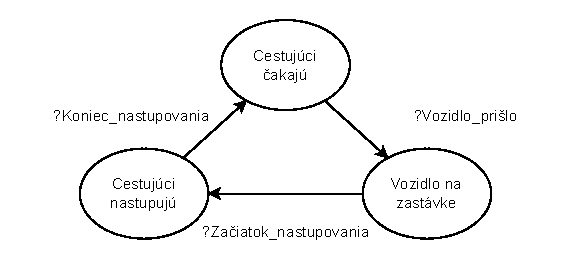
\includegraphics[width=0.6\textwidth]{DEVS-zastavka-sk.drawio.pdf}
  \caption{Stavový automat modelu zastávky}
\end{figure}

\begin{table}[h]\label{tab:stavy_zastavky}
  \centering
  \begin{tabularx}{\textwidth}{|l|X|}
    \hline
    \textbf{Stav} & \textbf{Popis} \\ \hline
    Cestujúci čakajú & na zastávke nie je žiadne vozidlo \\ \hline
    Vozidlo na zastávke & na zastávku práve prišlo vozidlo \\ \hline
    Cestujúci nastupujú & cestujúci nastupujú do vozidla \\ \hline
  \end{tabularx}
  \caption{Stavy modelu zastávky}
\end{table}

\begin{table}[h]\label{tab:inputs_zastavky}
  \centering
  \begin{tabularx}{\textwidth}{|l|X|}
    \hline
    \textbf{Vstupný signál} & \textbf{Akcia ktorú spúšťa} \\ \hline
    ?Vozidlo\_prišlo & výpočet časového intervalu medzi posledným príchodom a aktuálnym príchodom vozidla \\ \hline
    ?Začiatok\_nastupovania & generovanie príchodov cestujúcich \\ \hline
    ?Koniec\_nastupovania & prepísanie času posledného príchodu vozidla \\ \hline
  \end{tabularx}
  \caption{Vstupné signály modelu zastávky}
\end{table}

\subsubsection*{Generovanie príchodov cestujúcich}
Generovanie príchodov cestujúcich prebieha na základe exponenciálneho rozdelenia s parametrom $\lambda$ v časovom intervale medzi príchodom posledného a aktuálneho vozidla.
Tento parameter je v rámci jednej zastávky každú hodinu iný, pretože počet prichádzajúcich cestujúcich sa v priebehu dňa mení.
V algoritme~\ref{algoritmus_generovanie_cestujucich} je popísaný proces generovania príchodu cestujúcich na zastávku.
Ak by nám na správne fungovanie modelu stačil iba počet cestujúcich, na jeho výpočet by sme použili Poissonovo rozdelenie.
Pre výpočet doby čakania na zastávke je potrebné vedieť aj čas príchodu jednotlivých cestujúcich.
Preto je v simulačnom modeli použité exponenciálne rozdelenie, ktoré generuje náhodný časový interval medzi príchodami jednotlivých cestujúcich.
Vzťah medzi týmito dvoma rozdeleniami a podrobnejší popis exponenciálneho rozdelenia je v článku~\cite{geraghty2022exponential}.
Pripočítaním náhodného časového intervalu k aktuálnemu modelovému času sa vygeneruje čas príchodu cestujúceho, ktorý sa uloží do fronty predstavujúcej všetkých cestujúcich čakajúcich na zastávke.
Modelový čas sa zmení na čas príchodu cestujúceho.
Tento proces sa opakuje až kým modelový čas nedosiahne čas príchodu aktuálneho vozidla.

\vspace*{\dimexpr0.5\baselineskip\relax}
\begin{algorithm}[H]\label{algoritmus_generovanie_cestujucich}
\caption{Generovanie príchodov cestujúcich}
  získanie $\lambda$ pre danú zastávku a hodinu\;
  \While{modelový čas < čas príchodu vozidla} {
    vygenerovanie času príchodu cestujúceho\;
    pridanie cestujúceho do fronty\;
    zmena modelového času na čas príchodu cestujúceho\;
  }
\end{algorithm}

\newpage
\subsection*{Atomický model vozidla}\label{model_vozidla}

Každé vozidlo, respektíve jedna trasa, ktorú vozidlo podľa časového rozpisu prejde, je reprezentovaná jednou inštanciou modelu vozidla.

\[\langle S_i, q_{init,i}, {\delta}_{int,i}, ta_i, Y_i, {\lambda}_i, X_i, {\delta}_{ext,i} \rangle\]
\[S = \{\text{Na ceste}, \text{Na zastávke}, \text{Nakladá cestujúcich} \}\]
\[q_{init} = \text{Na ceste}\]
\[\delta_{int} = \{ \text{Na ceste} \rightarrow \text{Na zastávke}, \text{Na zastávke} \rightarrow \text{Nakladá cestujúcich},\]
\[\text{Nakladá cestujúcich} \rightarrow \text{Na ceste} \}\]
\[ta = \{ \text{Na ceste} \rightarrow \infty, \text{Na zastávke} \rightarrow 0, \text{Nakladá cestujúcich} \rightarrow 0 \}\]
\[Y = \{\text{\textit{!Príchod}}, \text{\textit{!Nastupovanie}}, \text{\textit{!Odchod}} \}\]
\[\lambda = \{ \text{Na ceste} \rightarrow \text{\textit{!Príchod}}, \text{Na zastávke} \rightarrow \text{\textit{!Nastupovanie}},\]
\[\text{Nakladá cestujúcich} \rightarrow \text{\textit{!Odchod}} \}\]
\[X = \{ \text{\textit{?Príchod\_vozidla}} \}\]
\[\delta_{ext} = \{ (\text{Na ceste, \textit{?Príchod\_vozidla}}) \rightarrow \text{Na zastávke} \}\]

Na obrázku~\ref{fig:model_vozidla} je graficky znázornený stavový automat modelu vozidla.
Zobrazuje tri stavy modelu a prechody medzi nimi, ktoré zároveň generujú tri výstupné signály.
Stavy modelu sú popísané v tabuľke~\ref{tab:stavy_vozidla} a akcie, ktoré sa vykonajú spolu s generovaním výstupných signálov sú popísané v tabuľke~\ref{tab:outputs_vozidla}.
Vo formálnej definícii vyššie je uvedené, že model vozidla zotrváva v stave \textbf{Na ceste} neobmedzene dlho.
Prechod z tohoto stavu je podmienený príchodom vstupného signálu \textit{?Príchod\_vozidla}.
Pôvod tohoto signálu bude popísaný v rámci definície zloženého modelu neskôr.

\begin{figure}[h]\label{fig:model_vozidla}
  \centering
  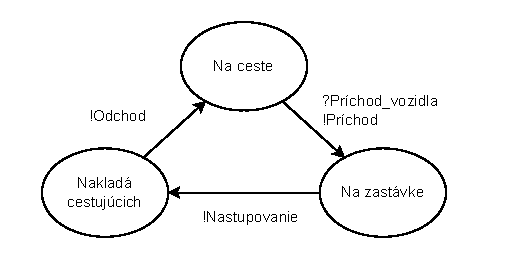
\includegraphics[width=0.6\textwidth]{DEVS-vozidlo-sk.drawio.pdf}
  \caption{Stavový automat modelu vozidla}
\end{figure}

\begin{table}[h]\label{tab:stavy_vozidla}
  \centering
  \begin{tabularx}{\textwidth}{|l|X|}
    \hline
    \textbf{Stav} & \textbf{Popis} \\ \hline
    Na ceste & vozidlo sa pohybuje medzi zastávkami \\ \hline
    Na zastávke & vozidlo práve prišlo na zastávku \\ \hline
    Nakladá cestujúcich & vozidlo nakladá cestujúcich \\ \hline % TODO zmenit nakalda cestujucich
  \end{tabularx}
  \caption{Stavy modelu vozidla}
\end{table}

\begin{table}[h]\label{tab:outputs_vozidla}
  \centering
  \begin{tabularx}{\textwidth}{|l|X|}
    \hline
    \textbf{Výstupný signál} & \textbf{Akcia ktorú spúšťa} \\ \hline
    !Príchod & výstup cestujúcich podľa koeficientu danej zastávky, napríklad ak je koeficient 0,7, vystúpi 70 percent cestujúcich \\ \hline
    !Nastupovanie & nástup cestujúcich do vozidla, tí ktorí sa nezmestia do vozidla sú nespokojní a následne opúšťajú systém \\ \hline % TODO zmenit nastupovanie
    !Odchod & okrem aktivácie prepojených vstupných signálov sa nič iné nevykonáva \\ \hline
  \end{tabularx}
  \caption{Výstupné signály modelu vozidla}
\end{table}

\subsubsection*{Obsluha zastávky}

Každé vozidlo začina na prvej zastávke v rozpise a počas simulácie sa musí pohybovať medzi zastávkami.
Proces, ktorý vozidlo vykoná pri príchode na každú zastávku, je popísaný v algoritme~\ref{algoritmus_obsluha_zastavky}.
Tento proces je vyvolaný príchodom vstupného signálu \textit{?Príchod\_vozidla}.

\vspace*{\dimexpr0.5\baselineskip\relax}
\begin{algorithm}[H]\label{algoritmus_obsluha_zastavky}
\caption{Obsluha zastávky}
  prepojenie výstupných signálov vozidla so vstupnými signálmi zastávky\;
  aktivácia výstupného signálu \textbf{!Príchod}\;
  aktivácia výstupného signálu \textbf{!Nastupovanie}\;
  aktivácia výstupného signálu \textbf{!Odchod}\;
\end{algorithm}

\newpage
\subsection*{Zložený model}
Zložený simulačný model v tejto práci pozostáva z dvoch atomických modelov, modelu zastávky a vozidla.
Prepojenie týchto atomických modelov je graficky znázornené na obrázku~\ref{fig:simulacny_model}.

\[D = \{ \text{Zastávka}, \text{Vozidlo} \}\]
\[M_{Zastávka} = \langle \ldots \rangle\] % TODO Zastávka Zastvka
\[M_{Vozidlo} = \langle \ldots \rangle\]
\[I_{Zastávka} = \emptyset\]
\[I_{Vozidlo} = \{ \text{Zastávka} \}\]
\[X_{self} = \emptyset\]
\[Y_{self} = \{ \text{\textit{!Príchod\_vozidla}} \}\]
\[\text{\textit{select}} = \{ \{Zastávka,Vozidlo\} \rightarrow Vozidlo, \{Zastávka\} \rightarrow Zastávka, \{Vozidlo\} \rightarrow Vozidlo \}\]
\[Z_{i,j,self} = \{ \text{\textit{!Príchod\_vozidla}} \rightarrow \text{\textit{?Príchod\_vozidla}},\]
\[\text{\textit{!Príchod}} \rightarrow \text{\textit{?Vozidlo\_prišlo}},\]
\[\text{\textit{!Nastupovanie}} \rightarrow \text{\textit{?Začiatok\_nastupovania}},\]
\[\text{\textit{!Odchod}} \rightarrow \text{\textit{?Koniec\_nastupovania}} \}\]

Samotný zložený model má navyše ešte jeden výstupný signál, ktorý je prepojený s modelom vozidla.
Týmto signálom sa spúšťa rutina obsluhy zastávky v rámci vozidla.
Vozidlo sa dostáva zo stavu \textbf{Na ceste} do stavu \textbf{Na zastávke}.
Výstupný signál zloženého modelu \textit{!Príchod\_vozidla} sa generuje pri spracovaní udalosti z kalenádara udalostí, oba tieto koncepty sú popísané neskôr.

\begin{figure}[h]\label{fig:simulacny_model}
  \centering
  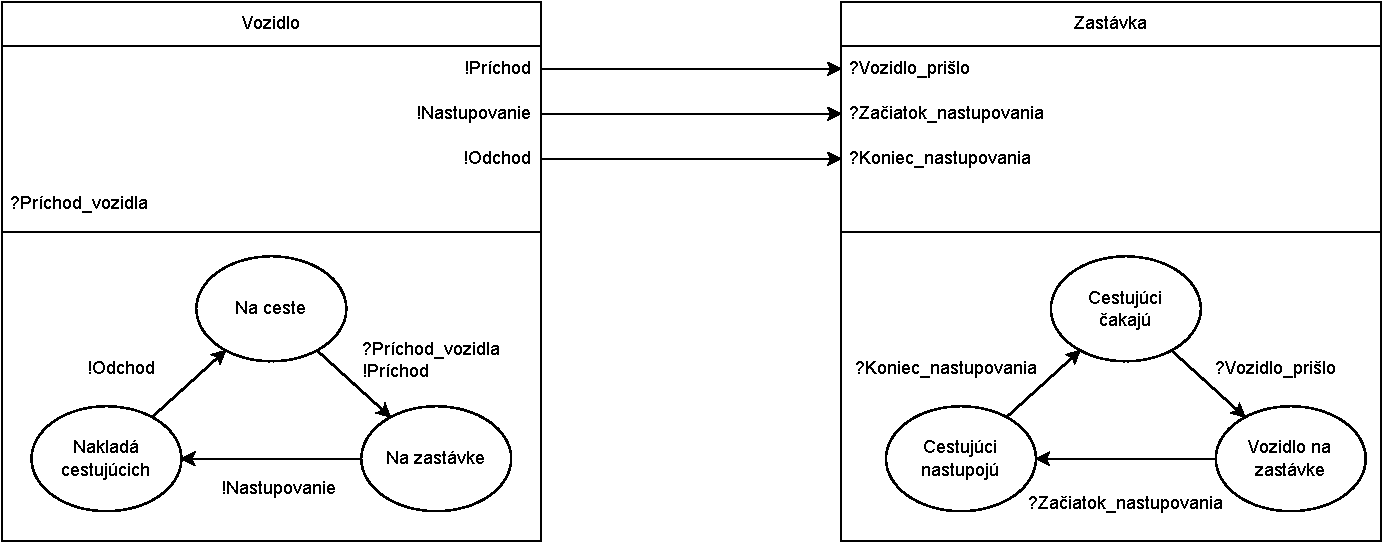
\includegraphics[width=\linewidth]{DEVS-sk.drawio.pdf}
  \caption{Schéma zloženého simulačného modelu}
\end{figure}

\subsection*{Udalosť príchodu vozidla na zastávku}
Udalosť príchodu vozidla na zastávku vyvolá spustenie rutiny obslúženia cestujúcich, ktorí čakajú na zastávke. Táto rutina je popísaná v algoritme~\ref{algoritmus_obsluha_zastavky}.
Parametre tejto udalosti sú:
\begin{itemize}
  \item \textbf{Čas príchodu} --- čas, kedy vozidlo prichádza na zastávku
  \item \textbf{Zastávka} --- zastávka, na ktorej sa udalosť vykonáva
  \item \textbf{Vozidlo} --- vozidlo, ktoré prichádza na zastávku
\end{itemize}

Vozidlo začína udalosť v stave \textbf{Na ceste}, príde na zastávku uvedenú v parametri udalosti, vykoná rutinu nástupu a výstupu cestujúcich a odchádza na ďalšiu zastávku.
Za jednu udalosť teda vozidlo prechádza všetkými svojimi vnútorným stavmi, udalosť končí opäť v stave \textbf{Na ceste}.
Zastávka, ktorá je uvedená v parametri udalosti, rovnako prechádza všetkými svojimi vnútornými stavmi vďaka prepojeniu výstupných signálov vozidla so vstupnými signálmi zastávky.

\subsection*{Kalendár udalostí}
Kalendár udalostí je základným prvkom modelu, ktorý riadi priebeh simulácie.
V kalendári sú uložené všetky udalosti, ktoré sa majú v modeli vykonať.
Vykonávané udalosti sú v prípade tohto modelu príchody vozidiel na zastávky.
V rámci jednej udalosti sa vykoná rutina obslúženia cestujúcich čakajúcich na zastávke.
Všetky udalosti sú naplánované na začiatku simulácie, pretože na základe časovému rozpisu sú presne definované všetky príchody vozidiel na jednotlivé zastávky.
Príchody na počiatočnú zastávku sú dané hlavným časovým rozpisom, príchody na ostatné zastávky sú odvodené od času potrebného na presun z jednej zastávky na následujúcu. % TODO zmenit prvu na pociatocnu
Pseudokód plánovania udalostí je uvedený v algoritme~\ref{algoritmus_planovanie_udalosti} a spolu s kódom v implementácii je prevzatý zo študijnej opory predmetu Modelovanie a simulácie~\cite{peringer2022ims}, ktorý je vyučovaný na Fakulte informatiky Vysokého učení technického v Brne.
V priebehu simulácie už nie je potrebné plánovať žiadne ďalšie udalosti.

\vspace*{\dimexpr0.5\baselineskip\relax}
\begin{algorithm}[H]\label{algoritmus_planovanie_udalosti}
  \caption{Plánovanie udalostí}
    \For{čas v časovom rozpise počiatočnej zastávky} {
      Vytvorí sa vozidlo (inicializuje sa objekt)\;
      \For{zastávka na linke} {
        Pridá sa udalosť príchodu vozidla na danú zastávku\;
      }
    }
\end{algorithm}
\vspace*{\dimexpr0.5\baselineskip\relax}

Po naplánovaní všetkých udalostí sa spustí simulácia.
Postupne sa vykonávajú jednotlivé udalosti a simulácia sa diskrétne posúva vpred dovtedy, až kým nie je kalendár udalostí prázdny alebo nie je dosiahnutý koncový čas simulácie.
Pseudokód riadenia simulácie je popísaný v algoritme~\ref{algoritmus_riadenia_simulacie}, teno kód je tiež prevzatý zo študijnej opory~\cite{peringer2022ims}.

\vspace*{\dimexpr0.5\baselineskip\relax}
\begin{algorithm}[H]\label{algoritmus_riadenia_simulacie}
\caption{Simulácia riadená udalosťami}
  \While{kalendár udalostí nie je prázdny} {
    Vyberie sa udalosť s najmenším časom v kalendári\;
    Udalosť sa odstráni z kalendára\;
    \If{čas udalosti > koncový čas simulácie} {
      Simulácia končí\;
    }
    Modelový čas sa nastaví na čas udalosti\;
    Udalosť sa vykoná (Vozidlo príde na zastávku a obslúži cestujúcich)\;
  }
\end{algorithm}
\vspace*{\dimexpr0.5\baselineskip\relax}

Pre potreby časového rozpisu stačí simulovať jeden deň.
V prípade rôznych rozpisov v čase pracovnýh dní a v čase sviatkov a víkendov sa jedná o kompletne iný rozpis, ktorý sa musí simulovať a optimalizovať samostatne.
Všetky naplánované udalsti by mali byť v rámci jedného dňa, preto simulácia vždy končí vyprázdnením kalendára udalostí a nie prekročením koncového času.

\section{Výstupy simulačného modelu}\label{vystupy_simulacneho_modelu}

Hlavný zmysel simulácie je postupné generovanie informácií, ktoré by sme inak museli získať z pozorovania reélnej prevádzky linky.
Efektivitu každého jedného časového rozpisu, ktorý program vytvorí, je potrebné otestovať a ohodnotiť, pre výber najlepšieho z nich, skôr ako ho začneme používať v reálnej prevádzke.
Na ohodnotenie jednotlivých rozpisov slúžia štatistiky získané počas simulácie.
Štatistiky sa zbierajú pre každú zastávku~\ref{tab:busStopStatistics_class}. aj pre každé vozidlo~\ref{tab:busStatistics_class} osobitne.
Následne sa agregujú do jednoho objektu \texttt{Statistics}, ktorého obsah je popísaný v tabuľke~\ref{tab:statistics_class}.
\begin{table}[h]\label{tab:statistics_class}
  \centering
  \begin{tabularx}{\textwidth}{|l|X|}
    \hline
    \textbf{Parameter} & \textbf{Popis} \\ \hline
    \texttt{totalNumberOfBuses} & Počet spojov v priebehu dňa na linke \\ \hline
    \texttt{busStopStatistics} & Agregované štatistiky zastávok \\ \hline
    \texttt{busStatistics} & Agregované štatistiky vozidiel \\ \hline
  \end{tabularx}
  \caption{Trieda \texttt{Statistics}}
\end{table}

\begin{table}[h]\label{tab:busStopStatistics_class}
  \centering
  \begin{tabularx}{\textwidth}{|l|X|}
    \hline
    \textbf{Parameter} & \textbf{Popis} \\ \hline
    \texttt{totalPassengersArrived} & Koľko cestujúcich prišlo na zastávku za deň \\ \hline
    \texttt{totalPassengersDeparted} & Koľko cestujúcich vytúpilo na zastávke za deň \\ \hline
    \texttt{totalPassengersLeftUnboarded} & Počet cestujúcich, ktorí sa nezmestili do vozidla \\ \hline
    \texttt{totalTimeSpentWaiting} & Čas, ktorý cestujúci strávili čakaním na zastávke \\ \hline
    \texttt{passengersArrivedPerHour} & Počet cestujúcich, ktorí prišli na zastávku za hodinu \\ \hline
    \texttt{passengersDepartedPerHour} & Počet cestujúcich, ktorí vystúpili na zastávke za hodinu \\ \hline
    \texttt{passengersLeftUnboardedPerHour} & Počet cestujúcich, ktorí sa nezmestili do vozidla za hodinu \\ \hline
    \texttt{timeSpentWaitingPerHour} & Čas, ktorý cestujúci strávili čakaním na zastávke za hodinu \\ \hline
  \end{tabularx}
  \caption{Trieda \texttt{busStopStatistics}}
\end{table}

\begin{table}[h]\label{tab:busStatistics_class}
  \centering
  \begin{tabularx}{\textwidth}{|l|X|}
    \hline
    \textbf{Parameter} & \textbf{Popis} \\ \hline
    \texttt{capacity} & Celková kapacita vozidla \\ \hline
    \texttt{seats} & Počet miest na sedenie \\ \hline
    \texttt{averageLoad} & Priemerná naplnenosť vozidla \\ \hline
    \texttt{averageLoadInPercent} & Priemerná naplnenosť vozidla v percentách \\ \hline
    \texttt{totalPassengersTransported} & Celkový počet prevezených cestujúcich \\ \hline
    \texttt{loadPerBusStop} & Naplnenosť vozidla na jednotlivých zastávkach \\ \hline
    \texttt{loadInPercentPerBusStop} & Naplnenosť vozidla na jednotlivých zastávkach v percentách \\ \hline
    \texttt{passengerSatisfactions} & Spokojnosť jednotlivých zákazníkov \\ \hline
  \end{tabularx}
  \caption{Trieda \texttt{busStatistics}}
\end{table}

\subsection*{Počet spojov v priebehu dňa na linke}
Tento údaj slúži pre optimalizáciu prevádzkových nákladov. Z pohľadu dopravného podniku je potrebné dosiahnuť, aby bol počet spojov čo najnižší.
Z pohľadu cestujúcich je potrebné aby bol počet spojov čo najväčší, aby nemuseli čakať dlho na spoj a estovali komfortne.
Preto je dôležité nájsť správny kompromis medzi týmito dvoma požiadavkami.

\subsection*{Koľko cestujúcich prišlo na zastávku za deň}
Celkový počet cestujúcich za deň je dobrým indikátorom toho, ako sú namáhané jednotlivé časti linky.
V prípadoch, kedy na zastávky v strede trasy prichádza oveľa viac cestujúcich ako na koncové zastávky, posilňuje dopravný podnik práve túto strednú časť ďalšími spojmi.

\subsection*{Koľko cestujúcich vystúpilo na zastávke za deň}
Je potrebné aby sme v rámci simulácie rátali aj s cestujúcimi, ktorí z vozidiel vystupujú, inak by sa kapacita vozidla hneď naplnila.
Ide o dôležitú časť reálneho systému, ktorú nemôžeme zanedbať ani pri simulácii.
Slúži na validáciu modelu.

\subsection*{Počet cestujúcich, ktorí sa nezmestili do vozidla}
Môže nastať situácia, že je vozidlo tak preplnené, že nie je možné aby všetci cestujúci čakajúci na zastávke do neho nastúpili.
Rozpisy, pri ktorých sa tento jav vyskytne, budú mať horšie hodnotenie.

\subsection*{Čas, ktorý cestujúci strávili čakaním na zastávke}
Čas, ktorý cestujúci strávili čakaním na zastávke sledujeme v dvoch rôznych údajoch, raz ako celkový čas čakania a raz ako priemerný čas čakania jedného cestujúceho.
V oboch prípadoch chceme, aby bol tento čas čo najnižší.

\subsection*{Počet cestujúcich, ktorí prišli na zastávku za hodinu}
Tento údaj má skôr informatívny charakter, pretože ide o vstup programu.
Algoritmus sa snaží vytvoriť rozpis, ktorý by bol schopný prepraviť všetkých cestujúcich.
Na grafe~\ref{fig:passengersArrivedPerHour} je vidieť, že v priebehu dňa sa počet cestujúcich prichádzajúcich na zastávku mení.
Obzvlášť v ranných a poobedných hodinách je tento počet výrazne vyšší ako počas dňa.
V týchto časoch by malo chodiť viac spojov.
\begin{figure}[h]\label{fig:passengersArrivedPerHour}
  \centering
  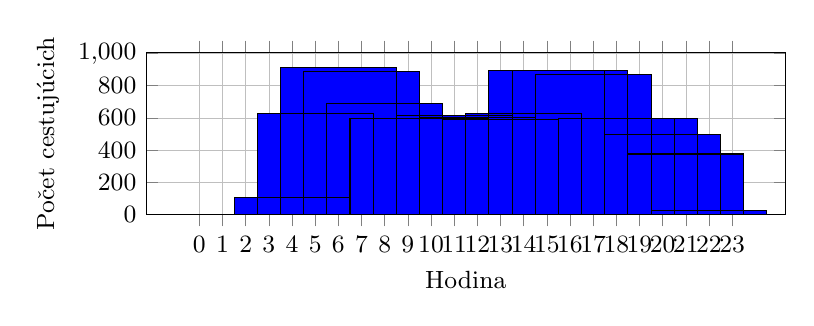
\begin{tikzpicture}
    \begin{axis}[
      width=0.8\textwidth,
      height=0.3\textwidth,
      xlabel={Hodina},
      ylabel={Počet cestujúcich},
      ymin=0,
      xtick={0,1,...,23},
      grid=both,
      major grid style={line width=.2pt,draw=gray!50},
      minor grid style={line width=.1pt,draw=gray!20},
      tick label style={font=\small},
      label style={font=\small},
      legend style={font=\small, at={(0.5,-0.2)}, anchor=north, legend columns=-1},
      ybar,
      bar width=5,
      ]
      \addplot[fill=blue] coordinates {
        (0, 0) (1, 0) (2, 0) (3, 0) (4, 104) (5, 625) (6, 915) (7, 888) 
        (8, 689) (9, 595) (10, 598) (11, 613) (12, 603) (13, 589) 
        (14, 630) (15, 894) (16, 897) (17, 872) (18, 597) (19, 597) 
        (20, 499) (21, 376) (22, 22) (23, 0)
      };
    \end{axis}
  \end{tikzpicture}
  \caption{Počet cestujúcich prichádzajúcich na zastávku za hodinu}
\end{figure}

\subsection*{Počet cestujúcich, ktorí vystúpili na zastávke za hodinu}
Jedná sa o rovnaký údaj ako je počet cestujúcich, ktorí vystúpili na zastávke za celý deň, ale rozdelený na jednotlivé hodiny dňa.

\subsection*{Počet cestujúcich, ktorí sa nezmestili do vozidla za hodinu}
Tento údaj informuje, že linka je v určitej časti dňa poddimenzovaná a bolo by vhodné v tomto čase linku posilniť.

\subsection*{Čas, ktorý cestujúci strávili čakaním na zastávke za hodinu}
Čas strávený čakaním na zastávke by mal byť počas celého dňa približne rovnaký.
Na grafe~\ref{fig:timeSpentWaitingPerHour} je vidieť ako sa priemerný čas čakania pohybuje v rozsahu približne 5 minút, ale o desiatej hodine večer tento čas náhle narastá.
Z uvedeného vyplíva, že by v tejto hodine malo byť nasadených viac vozidiel.
\begin{figure}[h]\label{fig:timeSpentWaitingPerHour}
  \centering
  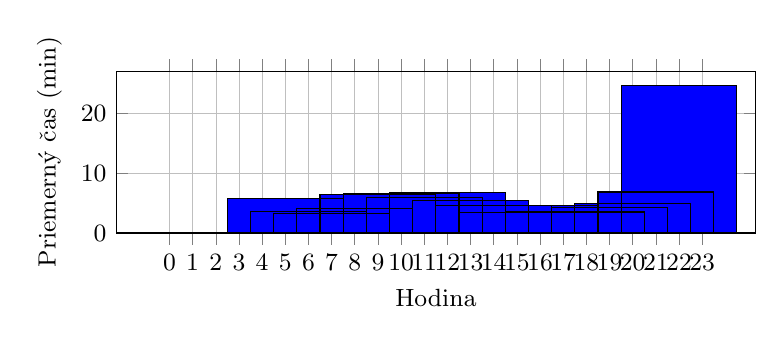
\begin{tikzpicture}
    \begin{axis}[
      width=0.8\textwidth,
      height=0.3\textwidth,
      xlabel={Hodina},
      ylabel={Priemerný čas (min)},
      ymin=0,
      xtick={0,1,...,23},
      grid=both,
      major grid style={line width=.2pt,draw=gray!50},
      minor grid style={line width=.1pt,draw=gray!20},
      tick label style={font=\small},
      label style={font=\small},
      legend style={font=\small, at={(0.5,-0.2)}, anchor=north, legend columns=-1},
      ybar,
      bar width=5,
      ]
      \addplot[fill=blue] coordinates {
        (0, 0) (1, 0) (2, 0) (3, 0) (4, 0) (5, 5.6816) (6, 3.5224043715846993) (7, 3.293918918918919) 
        (8, 4.0406386066763424) (9, 6.485714285714286) (10, 6.6003344481605355) (11, 5.993474714518761) 
        (12, 6.724709784411277) (13, 5.426146010186757) (14, 4.642857142857143) (15, 3.475391498881432) 
        (16, 4.517279821627648) (17, 3.5940366972477062) (18, 3.4974874371859297) (19, 4.239530988274707) 
        (20, 4.9318637274549095) (21, 6.843085106382978) (22, 24.545454545454547) (23, 0)
      };
    \end{axis}
  \end{tikzpicture}
  \caption{Priemerný čas strávený čakaním za hodinu}
\end{figure}

\subsection*{Celková kapacita vozidla}
Tento parameter je dôležitý, pretože na základe neho sa rozhoduje, koľko cestujúcich môže nastúpiť do vozidla.
Zároveň slúži pre výpočet naplnenosti vozidla v percentách.
Príliš malá alebo príliš veľká naplnenosť vozidla môže byť nežiadúca.

\subsection*{Počet miest na sedenie}
Počet miest na sedenie hrá rolu pri výpočte spokojnosti nastupujúceho cestujúceho.
Pokiaľ má možnosť si sadnúť, jeho spokojnosť bude vyššia, ako keby mal stáť.

\subsection*{Priemerná naplnenosť vozidla}
Priemerná naplnenosť vozidla je dôležitý parameter, ktorý nás informuje, ako veľmi sú vozidlá využívané.
Z pohľadu cestujúcich je lepšie, ak je vozidlo prázdnejšie, ale z pohľadu efektivity dopravného podniku je prázdnejšie vozidlo nevyužitý ekonomický potenciál.
Preto je potrebné nájsť kompromis medzi týmito dvoma požiadavkami.
Vyhodnotenie údaju priemernej naplnenosti vozidla a jeho optimalizácia je úlohou analytika dopravného podniku, ktorý môže tento výstup využívať pri svojej práci.

\subsection*{Celkový počet prevezených cestujúcich}
Celkový počet prevezených cestujúcich závisí od toho, koľko cestujúcich prišlo na jednotlivé zastávky a či sa im podarilo nastúpiť do jednotlivých vozidiel.
V ideálnom prípade sa tento počet bude rovnať celkovému počtu cestujúcich, ktorí prišli na zastávky.
V extrémnych prípadoch sa môže stať, že niektorí cestujúci zostanú na zastávkach a nenastúpia do žiadneho vozidla.

\subsection*{Naplnenosť vozidla na jednotlivých zastávkach}
Graf~\ref{fig:averageLoad} znázorňuje ako sa naplnenosť vozidiel mení počas ich jazdy.
Konkrétne sa jedná o linku 46 v Brne.
Naplnenosť sa postupne zvyšuje až kým nepríde na jednu z hlavných prestupných zastávok, Štefánikova čtvrť.
Tu vystúpi veľké množstvo cestujúcich a naplnenosť vozidla sa zníži.
Pokiaľ má linka príliš veľké výkyvy v naplnenosti vozidiel počas svojej trasy, je to znakom toho, že je potrebné trasu na určitých úsekoch posilniť inou linkou.
\begin{figure}[h]\label{fig:averageLoad}
  \centering
  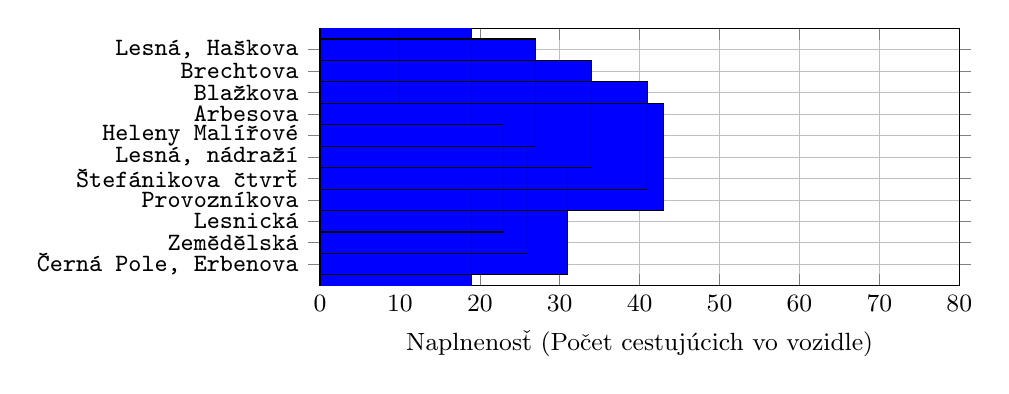
\begin{tikzpicture}
    \begin{axis}[
      width=0.8\textwidth,
      height=0.4\textwidth,
      xlabel={Naplnenosť (Počet cestujúcich vo vozidle)},
      xmin=0, xmax=80,
      ytick={1,2,...,11},
      yticklabels={
        \texttt{Černá Pole, Erbenova},
        \texttt{Zemědělská},
        \texttt{Lesnická},
        \texttt{Provozníkova},
        \texttt{Štefánikova čtvrť},
        \texttt{Lesná, nádraží},
        \texttt{Heleny Malířové},
        \texttt{Arbesova},
        \texttt{Blažkova},
        \texttt{Brechtova},
        \texttt{Lesná, Haškova}
      },
      grid=both,
      major grid style={line width=.2pt,draw=gray!50},
      minor grid style={line width=.1pt,draw=gray!20},
      tick label style={font=\small},
      label style={font=\small},
      legend style={font=\small, at={(0.5,-0.15)}, anchor=north, legend columns=-1},
      xbar,
      bar width=5,
      ]
      \addplot[fill=blue] coordinates {
        (0, 1) (19, 2) (31, 3) (26, 4) (23, 5) (43, 6) (41, 7) (34, 8) 
        (27, 9) (19, 10) (10, 11)
      };
    \end{axis}
  \end{tikzpicture}
  \caption{Priemerná naplnenosť vozidla na jednotlivých zastávkach linky 46}
\end{figure}

\subsection*{Spokojnosť jednotlivých zákazníkov}
Spokojnosť jednotlivých zákazníkov je klúčová pri optimalizácii časového rozpisu, na základe nej sa rozpis ohodnocuje.
Spokojnosť program počíta za každého cestujúceho a nakoniec program vypočíta priemer za celý deň.

\chapter{Optimalizácia časového rozpisu linky mestskej hormadnej dopravy}\label{optimalizacia}

Táto kapitola pojednáva o potrebných vstupoch, obmedzeniach, použitej optimalizačnej metóde a výstupoch optimalizácie.

Na optimalizáciu časového rozpisu bol použitý genetický algoritmus.
Genetický algoritmus je heuristická optimalizačná metóda, ktorá sa inšpiruje evolučnou biológiou.
Je založená na princípe prírodného výberu, kde sa najlepšie jedince z populácie vyberajú na reprodukciu a vytvárajú novú generáciu.
Vlastnosti jedincov by sa mali v priebehu generácií zlepšovať, až kým sa nenájde optimálne riešenie.
Okrem nájdenia optimálneho riešenia, môže byť genetický algoritmus ukončený aj dosiahnutím maximálneho počtu generácií alebo stagnáciou kvality riešenia.
Na ohodnotenie jedinca sa používa takzvaná fitness funkcia, ktorá hodnotí kvalitu riešenia na základe zadaných kritérií.
V prípade časových rozpisov MHD sa na výpočet fitness funkcie používajú štatistiky zo simulácie, ktoré sú popísané v kapitole~\ref{vystupy_simulacneho_modelu}.

\section{Potrebné používateľské vstupy}\label{vstupy_pouzivatela}
Pre správne fungovanie algoritmu, je potrebné zadať niekoľko povinných vstupných parametrov týkajúcich sa zastávok, linky a samotného genetického algoritmu.

\subsubsection{Vstupné parametre zastávky}
\begin{itemize}
  \item \textbf{Názov zastávky} --- názov zastávky, zobrazovaný na výstupoch
  \item \textbf{Čas príchodu} --- predpokladaný čas potrebný na prejazd od počiatočnej zastávky
  \item \textbf{Štatistika o príchodoch cestujúcich} --- priemerný počet prichádzajúcich cestujúcich v každej hodine dňa
  \item \textbf{Pravdepodobnosť výstupu cestujúceho} --- koeficient potrebný pre priebežné vyprázdnenie vozidla
\end{itemize}
Tieto informácie sa importujú formou textového súboru, každá zastávka je na samostatnom riadku a jednotlivé údaje sú oddelené dvojbodkou.

Vzor formátu importovaného súboru:

\noindent \texttt{Lesná, Haškova:0:[(5, 60), (6, 90), \ldots , (21, 40), (22, 30)]:0 \newline
  Brechtova:1:[(5, 60), (6, 90), \ldots , (21, 40), (22, 30)]:0.1 \newline
  Blažkova:2:[(5, 60), (6, 90), \ldots , (21, 40), (22, 30)]:0.1 \newline
  \ldots
}

\subsubsection{Vstupné parametre linky}
\begin{itemize}
  \item \textbf{Kapacita vozidla} --- maximálny možný počet cestujúcich vo vozidle
  \item \textbf{Miesta na sedenie} --- počet miest na sedenie vo vozidle
  \item \textbf{Celkové náklady} --- udávané v korunách na 100 miestokilometrov (vysvetlné v sekcii~\ref{fitness})  
  \item \textbf{Dĺžka trasy} --- dĺžka trasy v kilometroch
\end{itemize}
Kapacita vozidla a počet miest na sedenie sú potrebné pre výpočet naplnenosti vozidla, od ktorej sa potom odvíja spokojnosť cestujúcich.
Celkové náklady na 100 miestokilometrov a dĺžka trasy sú potrebné pre výpočet nákladov na prevádzku linky.
Podrobnejší popis výpočtu celkovej spokojnosti a nákladov na prevádzku je v kapitole~\ref{fitness}.

\subsubsection{Vstupné parametre genetického algoritmu}
\begin{itemize}
  \item \textbf{Veľkosť populácie} --- počet jedincov (časových rozpisov) v jednej generácii genetického algoritmu
  \item \textbf{Počet generácií} --- počet generácií, ktoré sa majú algoritmom vykonať
  \item \textbf{Pravdepodobnosť mutácie} --- pravdepodobnosť, že sa v jedincovi vyskytne mutácia
  \item \textbf{Maximálny počet spojov za hodinu} --- maximálny počet spojov, ktorý môže byť vygenerovaný za hodinu
\end{itemize}

\subsubsection{Vstupné obmedzenia časového rozpisu}
Poslednou informáciou, ktorá je od používateľa potrebná je obmedzenie počtu spojov za hodinu.
Používateľ takto môže nastavuje fixný počet spojov, ktorý sa musí vygenerovať za hodinu.
Toto obmedzenie sa využíva hľavne pri plánovaní náväznosti liniek, kedy je potrebné, aby sa niektoré spoje stretli na prestupnej zastávke.
Obvykle sa to robí tak, že sa nastaví rovnaký počet spojov pre všetky prestupné linky, ktoré sa na tejto zastávke stretávajú.

Toto obmedzenie je využívané aj v predbežnej analýze, ktorá sa vykonáva pred optimalizáciou.
V prípade že pre niektorú hodinu neexistuje údaj o priemernom počte prichádzajúcich cestujúcich na všetky zastávky linky, automaticky sa nastaví fixný počet spojov v danej hodine na 0 (napríklad nočná linka nepremáva cez deň).
Zadaním vstupných ombedzení časového rozpisu sa znižuje náročnosť výpočtu a zvyšuje kvalita nájdeného riešenia.

\section{Základná implementácia genetického algoritmu}\label{implementacia_genetickeho_algoritmu}
Na optimalizáciu časového rozpisu bol použitý genetický algoritmus.
Genetický algoritmus je heuristická optimalizačná metóda, ktorá sa inšpiruje Darwinovou teóriou evolúcie.
Podľa citátu od Charlesa Darwina, "V prírode je prežitie a úspech otázkou tých najschopnejších a najpríťažlivejších",
aj genetický algoritmus sa snaží nájsť najlepšie riešenie pomocou evolučného procesu.

Používajú sa postupy ako náhodná mutácia jedinca, rôzne typy výberu a kríženia jedincov.
Základnou premysou je, že najlepší jedinci v generácii buď splňujú zadané požiadavky alebo sú veľmi blízko k ich splneniu.
Predpokladá sa, že týto jedinci majú najvhodnejšie predispozície na to, aby ich potomkovia lepšie spĺňali zadané podmienky.
Využitie genetického algoritmu je efektívne v prípadoch, kedy by deterministické metódy trvali príliš dlho alebo by vôbec neboli schopné nájsť optimálne riešenie.
Genetický algoritmus bol prvýkrát predstavený okolo roku 1960 Johnom Hollandom na Univerzite v Michigane.
Uvedené informácie sú prevzaté zo zborníku z konferencie ICCES 2019~\cite{immanuel2019genetic}.

\vspace*{\dimexpr0.5\baselineskip\relax}
\begin{algorithm}[H]\label{algoritmus_geneticky_algoritmus}
\caption{Genetický algoritmus}
  Inicializácia prvej populácie\;
  Definovanie fitness funkcie\;
  Výpočet fitness funkcie pre každého jedinca v populácii\;
  \While{nie je nájdené optimálne riešenie alebo nebol dosiahnutý maximálny počet generácií} {
    Výber rodičov z populácie\;
    Kríženie rodičov na vytvorenie potomkov\;
    Mutácia potomkov\;
    Výpočet fitness funkcie pre každého potomka\;
  }
  Výber najlepšieho jedinca z populácie\;
\end{algorithm}
\vspace*{\dimexpr0.5\baselineskip\relax}

V prípade optimalizácie časového rozpisu MHD sa jedincami stávajú samotné časové rozpisy.
Na základe simulácie jedného dňa na linke s použitým časovým rozpisom sa získajú štatistiky, ktoré sa následne použijú na ohodnotenie kvality jedinca.

\subsection*{Reprezentácia jedinca}
V genetickom algoritme je jedinec reprezentovaný takzvaným chromozómom.
Chromozóm je reťazec génov, informácií o jedincovi.
V prípade časového rozpisu MHD je chromozómom pole obsahujúce 24 čísel (viď tabuľku~\ref{tab:chromosome}), ktoré predstavujú počet odchodov vozidiel z počiatočnej zastávky linky v jednotlivých hodinách dňa.

\begin{table}[h]\label{tab:chromosome}
  \centering
  \begin{tabularx}{\textwidth}{|l|X|X|X|X|X|X|X|X|X|X|X|X|X|X|X|X|X|X|X|X|X|X|X|X|}
    \hline
    0 & 0 & 0 & 0 & 0 & 5 & 7 & 9 & 9 & 9 & 7 & 6 & 6 & 6 & 6 & 7 & 9 & 9 & 7 & 7 & 6 & 5 & 4 & 3 \\ \hline
  \end{tabularx}
  \caption{Príklad chromozómu}
\end{table}

\subsection*{Fitness funkcia --- výpočet cieľov}\label{fitness}
Pre ohodnotenie kvality časového rozpisu boli definované dva hlavné ciele:
\begin{itemize}
  \item \textbf{Spokojnosť cestujúcich} --- priemerné percentuálne hodnotenie spokojnosti všetkých cestujúcich, ktorí prišli za daný deň na zastávku
  \item \textbf{Náklady na prevádzku} --- celkové náklady na prevádzku linky za deň, udávané v korunách na 100 miestokilometrov
\end{itemize}

Výpočet spokojnosti cestujúceho sa vykonáva v čase nástupu do vozidla. Hodnotí sa aktuálna naplnenosť vozidla, na základe ktorej sa vypočíta percentuálne hodnotenie spokojnosti.
Potrebné parametre pre výpočet sú kapacita vozidla, počet miest na sedenie a aktuálna naplnenosť vozidla.

Výpočet sa riadi následujúcimi troma podmienkami:
\begin{enumerate}
  \item Ak sú vo vozidle voľné miesta na sedenie, cestujúci si sadne a jeho spokojnosť je 1
  \item Ak je vozidlo úplne plné a cestujúci sa do neho nezmestí, jeho spokojnosť je 0
  \item Ak je vo vozidle miesto, ale už len na státie, spokojnosť vozidla závisí od aktuálnej naplnenosti cestujúceho a je vypočítaná podľa rovnice~\ref{eq_spokojnost} následovne: \begin{equation}\label{eq_spokojnost}
      \text{spokojnosť} = 1 - \frac{\text{aktualna naplnenosť vozidla} - \text{počet miest na sedenie}}{\text{kapacita vozidla}  - \text{počet miest na sedenie}}
    \end{equation}
\end{enumerate}
Spokojnosť všetkých cestujúcich sa vypočíta ako priemer spokojnosti jednotlivých cestujúcich.
Hodnota spokojnosti sa pohybuje od 0 do 1 a genetický algoritmus automaticky uprednostňuje vyššie hodnoty, teda dosiahnutie vyššej spokojnosti u cestujúcich.
\vspace*{\dimexpr0.5\baselineskip\relax}

Celkové náklady na prevádzku linky sú vypočítané z počtu a kapacity použitých vozidiel v časovom rozpise, dĺžky trasy a nákladov na jeden miestokilometer.
Jeden miestokilometer je definovaný ako vzdialenosť jedného kilometra, ktorú prejde jedno miesto vo vozidle~\cite{iata_rpks_asks}.
Napríklad vozidlo s kapacitu 80 miest, ktoré prejde 10 kilometrov, prejde 800 miestokilometrov.
Miestokilometre sa môžu násobiť aj počtom vozidiel, potom dve takéto vozidlá by prešli 1600 miestokilometrov.
Miestokilometer je potrebný pre výpočet efektivity linky, pretože náklady vo finančnom pláne Dopravného podniku mesta Brno sú udávané v českých korunách na 100 miestokilometrov.
Tento finančný plán je súčasťou zmluvy medzi mestom Brno a Dopravným podníkom mesta Brna~\cite{brno_dpmb_smlouva_2023}.
Celý výpočet nákladov na prevádzku linky teda závisí od štyroch premenných a je daný rovnicou~\ref{eq_naklady}:
\begin{equation}\label{eq_naklady}
  \text{celkové náklady} = \frac{\text{dĺžka trasy} \cdot \text{počet spojov} \cdot \text{kapacita vozidla}}{100} \cdot \text{náklady}
\end{equation}

Tieto dva ciele sú v neustálom konflikte --- viac spojov na linke a vyššia spokojnosť cestujúcich voči rastúcim nákladom na prevádzku DPMB.
Túto situáciu rieši multi-objektívna optimalizácia, ktorá sa snaží nájsť optimálne riešenie pre oba ciele naraz.

\subsection*{Genetický algoritmus s viacerými cieľmi}
Genetický algoritmus, ktorým sa snažíme dosiahnuť optimálneho kompromisu medzi viacerými cieľmi sa nazýva multi-objektívny genetický algoritmus.
Jeho podstata spočíva v nájdení Pareto frontu, čo je množina všetkých možných riešení, ktoré sú optimálne z pohľadu všetkých cieľov.
To znamená, že neexistuje žiaden iný jedinec, ktorý by bol lepší v oboch cieľoch naraz.

Ak existuje jeden jedinec, ktorý je lepší v oboch cieľoch, hovoríme, že dominuje iného jedinca.
V prípade, že dominuje iba v jednom cieli, ale v druhom nie, patria do rovnakej skupiny --- sú si rovnocenní.
Ak je jedinec horší v oboch cieľoch, hovoríme, že je dominovaný.
Každá generácia sa rozdelí do rovnocenných skupín, pri výbere rodičov sa uprednostňujú jedinci z lepšej skupiny.
Algoritmus sa snaží nájsť Pareto front, množinu tých najlepších možných jedincov.
Postupnou evolúciou jedinci získavajú lepšie vlastnosti a čím novšia je generácia, tým viac sa približuje k hľadanému Pareto frontu.
Na obrázku~\ref{fig:pareto_front} je znázornený Pareto front pre dva ciele, spokojnosť a náklady.
Multi-objektívne genetické algoritmy dokážu pracovať aj s viac ako dvoma cieľmi.
Pre optimalizáciu časového rozpisu však stačia dva, jeden zo strany zákazníka (spokojnosť) a druhý zo strany dopravného podniku (náklady).
Tieto základné informácie o fungovaní multi-objektívnych genetických algoritmov s použitím Pareto frontu boli prevzaté z článku~\cite{ngatchou2005pareto}.

\begin{figure}[h]\label{fig:pareto_front}
  \centering
  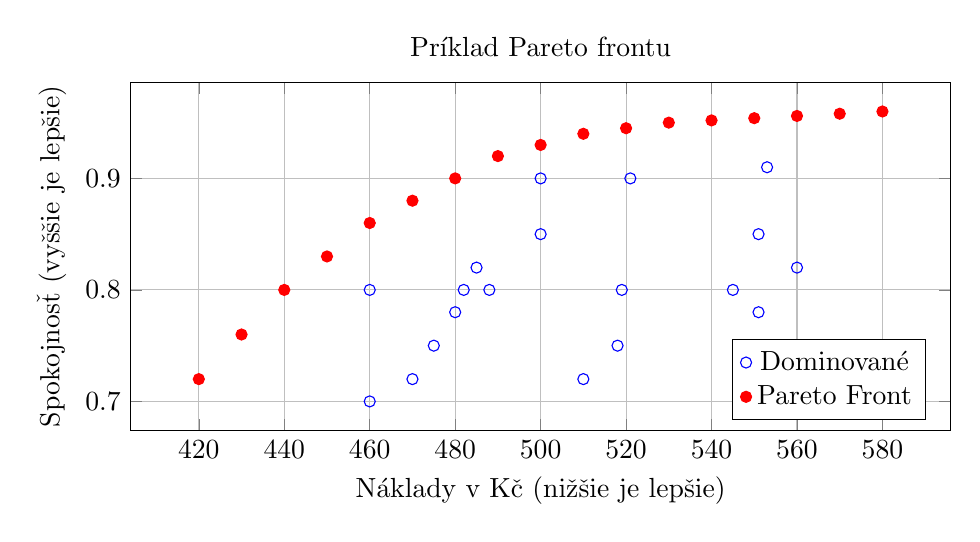
\begin{tikzpicture}
    \begin{axis}[
      xlabel={Náklady v Kč (nižšie je lepšie)},
      ylabel={Spokojnosť (vyššie je lepšie)},
      title={Príklad Pareto frontu},
      grid=major,
      legend pos=south east,
      width=12cm,
      height=6cm,
      scatter/classes={
        dominated={mark=o,draw=blue},
        pareto={mark=*,draw=red,fill=red}
      }
    ]
    \addplot[
      scatter,
      only marks,
      scatter src=explicit symbolic
    ]
    table[meta=label] {
      x y label
      420.0 0.72 pareto
      430.0 0.76 pareto
      440.0 0.80 pareto
      450.0 0.83 pareto
      460.0 0.86 pareto
      470.0 0.88 pareto
      480.0 0.9 pareto
      490.0 0.92 pareto
      500.0 0.93 pareto
      510.0 0.94 pareto
      520.0 0.945 pareto
      530.0 0.95 pareto
      540.0 0.952 pareto
      550.0 0.954 pareto
      560.0 0.956 pareto
      570.0 0.958 pareto
      580.0 0.96 pareto

      460.0 0.70 dominated
      470.0 0.72 dominated
      460.0 0.8 dominated
      475.0 0.75 dominated
      480.0 0.78 dominated
      482.0 0.80 dominated
      485.0 0.82 dominated
      488.0 0.80 dominated
      500.0 0.90 dominated
      500.0 0.85 dominated
      510.0 0.72 dominated
      518.0 0.75 dominated
      519.0 0.80 dominated
      521.0 0.90 dominated
      545.0 0.80 dominated
      547.0 0.75 dominated
      550.0 0.70 dominated
      551.0 0.78 dominated
      551.0 0.85 dominated
      553.0 0.91 dominated
      560.0 0.82 dominated
      580.0 0.75 dominated
    };
    \legend{Dominované, Pareto Front}
    \end{axis}
  \end{tikzpicture}
  \caption{Príklad Pareto frontu}
\end{figure}

\section{Multi-objektívny genetický algoritmus}

Pre účely multi-objektívnej optimalizácie bol použitý algoritmus NSGA-II (Non-dominated Sorting Genetic Algorithm II).
V článku~\cite{deb2002nsga} je porovnanie tohto algoritmu s inými multi-objektívnymi genetickými algoritmami.
NSGA-II vo viacerých testoch preukázal, že má lepšie rozloženie a diverzitu jedincov v Pareto fronte ako iné algoritmy.
Práve pre túto vlastnosť bol zvolený aj pre optimalizáciu časového rozpisu.
Okrem testov je v článku~\cite{deb2002nsga} aj podrobný popis fungovania algoritmu.
Algoritmy~\ref{algoritmus_nsga2},~\ref{algoritmus_non_dominated_sorting},~\ref{algoritmus_crowding_distance_assignment} a~\ref{algoritmus_comparsion_operator} boli z tohto článku prevzaté a mierne upravené pre naše účely.

NSGA-II je založený na triedení jedincov do frontov na základe ich dominancie nad inými jedincami.
Pri výbere jedincov pri krížení sa uprednostňujú jedinci z lepších frontov.
V prípade, že treba porovnať dvoch jedincov z rovnakého frontu, použije sa zhluková vzdialenosť.

Zhluková vzdialenosť zaisťuje vysokú diverzitu jedincov, pretože sa uprednostňujú jedinci, ktorí sú od seba najďalej, teda majú veľké rozdiely v hodnotách cieľov.
Pre jej výpočet sa najprv jedinci frontu zoradia podľa hodnoty jedného z cieľov.
Zhluková vzdialenosť daného jedinca pre daný cieľ je pomer medzi vzdialenosťami jedinca od jeho susedov vo fronte a vzdialenosťou medzi prvým a posledným jedincom vo fronte.
Zhlukové vzdialenosti pre jednotlivé ciele sa následne sčítajú a tým sa získa celková zhluková vzdialenosť jedinca.
Celý postup pre priradenie zhlukovej vzdialenosti je popísaný v algoritme~\ref{algoritmus_crowding_distance_assignment}.

Oproti klasickému genetickému algoritmu NSGA-II spracováva elitizmus inak.
V NSGA-II neexistuje konštanta, ktorá by udávala počet elitných jedincov, ktorí sa prenesú do ďalšej generácie.
Pri vytváraní novej generácie sa najprv vytvorí nová populácia z rodičov a ich potomkov.
Táto, dvojnásobne veľká populácia sa následne rozdelí do frontov a pre každého jedinca sa vypočíta zhluková vzdialenosť na základe jeho vzdialenosti od svojich susedov vo fronte.
Potom sa najepšie fronty prenesú do novej generácie.
Posledný prenášaný front sa pravdepodobne do novej generácie nezmestí celý, vtedy sa vyberie toľko jedincov z daného frontu, aby bola populácia rovnako veľká naprieč všetkými generáciami.
Jedinci z posledného frontu sa vyberajú na základe zhlukovej vzdialenosti, aby sa zachovala vyššia diverzita.

\subsection*{Rýchle nedominantné triedenie}
Rýchle nedominantné triedenie je základom NSGA-II.
Triedi jedincov do frontov na základe ich dominancie nad inými jedincami.
Jedince, ktoré sa navzájom nedominujú, patria do rovnakej skupiny, frontu, preto sa toto triedenie nazýva nedominantné.
Triedenie sa vykonáva v dvoch krokoch.
V prvom kroku sa musia porovnať všetci jedinci navzájom.
Pre každého jedinca $p$ v prvom cykle algoritmu~\ref{algoritmus_non_dominated_sorting} sa vypočíta množina $S_p$, ktorá obsahuje všetkých jedincov, ktorých dominuje $p$ a počet $n_p$, ktorý udáva počet jedincov, ktorí dominujú $p$.
Pokiaľ je $n_p = 0$, jedinec $p$ je nie je nikým dominovaný a pripojí sa do prvého frontu.
Taktiež sa mu priradí hodnota $p_{rank} = 1$.
Rank je hodnota, ktorá udáva v akom fronte sa jedinec nachádza, čím nižšia hodnota, tým je jedinec lepší.

Následuje druhý hlavný cyklus algoritmu~\ref{algoritmus_non_dominated_sorting}, ktorý vytvorí zvyšné fronty.
Princíp je taký, že pre každého jedinca $p$ v posledne vytvorenom fronte sa upravia hodnoty $n_q$ všetkých jedincov $q$ z množiny $S_p$.
To vpodstate znamená odstránenie jedinca $p$ z riešeného problému.
Na konci tohto cyklu by sa mal z problému odstrániť celý front $F_i$.
To znamená, že niektorí jedinci by sa mali stať tými najlepšími v tomto obmedzenom probléme.
Práve títo jedinci sa pridajú do ďalšieho frontu $F_{i+1}$.
Tento cyklus sa opakuje až pokým sa do najnovšieho frontu nemá kto pridať.

Toto triedenie teda iteratívne nachádza najlepší front a odstraňuje ho z problému až pokým sa nenájdu všetky fronty.

\vspace*{\dimexpr0.5\baselineskip\relax}
\begin{algorithm}[h]\label{algoritmus_non_dominated_sorting}
\caption{Rýchle nedominantné triedenie}
\KwIn{Populácia $P$}
\KwOut{Fronty nedominovaných jedincov $F$}
  $F \gets \emptyset$ (množina frontov)\;
  \For{každý jedinec $p \in P$} {
    $S_p \gets \emptyset$ (množina jedincov, ktorých dominuje $p$)\;
    $n_p \gets 0$ (počet jedincov, ktorí dominujú $p$)\;
    \For{každý jedinec $q \in P: q \neq p$} {
      \If{$p$ dominuje $q$} {
        $S_p \gets S_p \cup \{q\}$\;
      }
      \ElseIf{$q$ dominuje $p$} {
        $n_p \gets n_p + 1$\;
      }
    }
    \If{$n_p = 0$} {
      $p_{rank} \gets 1$\;
      $F_1 \gets F_1 \cup \{p\}$ (pridanie jedinca $p$ do prvého frontu)\;
    }
  }
  $i \gets 1$\;
  \While{$F_i \neq \emptyset$} {
    $Q \gets \emptyset$ (množina jedincov ďalšieho frontu)\;
    \For{každý jedinec $p \in F_i$} {
      \For{každý jedinec $q \in S_p$} {
        $n_q \gets n_q - 1$\;
        \If{$n_q = 0$} {
          $q_{rank} \gets i + 1$\;
          $Q \gets Q \cup \{q\}$\;
        }
      }
    }
    $i \gets i + 1$\;
    $F_i \gets Q$\;
  }
  \Return $F$\;
\end{algorithm}

\subsection*{Priradenie zhlukovej vzdialenosti}
V rámci jednoho frontu sa jedinci porovnávajú na základe zhlukovej vzdialenosti.
Zhluková vzdialenosť je definovaná ako vzdialenosť jedinca od jeho susedov vo fronte.
Vypočítava sa pre každý cieľ zvlášť a následne sa spočíta.
Najdôležitejšou časťou algoritmu~\ref{algoritmus_crowding_distance_assignment} je cyklus, ktorý sa vykonáva pre každý cieľ $c$, teda v prípade optimalizácie časového rozpisu pre spokojnosť zákazníkov a celkové náklady.
Výpočet hodnôt oboch cieľov je popísaný v sekcii~\ref{implementacia_genetickeho_algoritmu}.
Najprv sa jedinci zoradia podľa dosiahnutých hodnôt cieľa $c$.
Následne sa vytýčia krajné body, jedincom s najmenšou a najväčšou hodnotou cieľa $c$ sa priradí nekonečná zhluková vzdialenosť, pretože sú najviac diverzní.
Pre všetkých ostatných jedincov vo fronte a pre cieľ $c$ sa vypočíta zhluková vzdialenosť ako podiel rozdielu hodnôt susedov a rozdielu krajných jedincov.
Tieto čiastočné vzdialenosti sa postupne sčítavajú do celkovej zhlukovej vzdialenosti jedinca.

\vspace*{\dimexpr0.5\baselineskip\relax}
\begin{algorithm}[h]\label{algoritmus_crowding_distance_assignment}
\caption{Priradenie zhlukovej vzdialenosti}
\KwIn{Front $L$}
  $l \gets |L|$ (počet jedincov frontu)\;
  \For{každý jedinec $p \in L$} {
    $p_{vzdialenost} \gets 0$ (inicializácia zhlukovej vzdialenosti)\;
  }
  \For{každý cieľ $c$} {
    $L \gets sort(L, c)$ (zoradenie jedincov podľa hodnôt cieľa $c$)\;
    $L[0] \gets \infty$ (priradenie nekonečnej vzdialenosti najmenšiemu jedincovi)\;
    $L[l-1] \gets \infty$ (priradenie nekonečnej vzdialenosti najväčšiemu jedincovi)\;
    \For{$i = 1$ do $l - 2$} {
      $L[i]_{vzdialenost} \gets L[i]_{vzdialenost} + \frac{L[i+1].c - L[i-1].c}{L[l-1].c - L[0].c}$\;
    }
  }
\end{algorithm}

\subsection*{Porovnávací operátor $\prec_n$}
Informácie získané z rýchleho nedominantného triedenia~\ref{algoritmus_non_dominated_sorting} a priradenia zhlukovej vzdialenosti~\ref{algoritmus_crowding_distance_assignment} sa použijú na porovnanie dvoch jedincov.
Pokiaľ je jedinec $p$ z lepšieho frontu ako jedinec $q$, teda má lepší, nižší rank, $p$ dominuje $q$.
Ak sú jedinci z rovnakého frontu, porovnávajú sa na základe zhlukovej vzdialenosti.
Dominuje ten, ktorý má väčšiu zhlukovú vzdialenosť, to znamená, že sa výraznejšie odlišuje od svojich susedov vo fronte.
Tento porovnávací operátor je znázornený v algoritme~\ref{algoritmus_comparsion_operator}.

\vspace*{\dimexpr0.5\baselineskip\relax}
\begin{algorithm}[h]\label{algoritmus_comparsion_operator}
\caption{Porovnávací operátor $\prec_n$}
\KwIn{Jedinci $p$ a $q$}
\KwOut{True ak $p$ dominuje $q$, inak False}
  \Return $p_{rank} < q_{rank} \vee (p_{rank} = q_{rank} \wedge p_{vzdialenost} > q_{vzdialenost})$\;
  (dá sa rozšíriť aj o obmedzenia)\;
\end{algorithm}

Toto porovnávanie sa dá rozšíriť aj o rôzne obmedzenia.
Napríklad, v rámci optimalizácie časového rozpisu máme dva cieľe, spokojnosť zákazníkov a celkové náklady, ale porovnávanie sme rozšírili o to, v ktorom rozpise dôjde menej často k úplnému preplneniu vozidla.
Sledujeme počet prípadov, kedy sa nejaký cestujúci nezmestil do vozidla.
V prípade, že aspoň jeden z porovnávaných jedincov má tento počet väčší ako 0, vyhráva ten, ktorý má tento počet nižší.
Všeobecne môže byť obmedzení aj viac, v takom prípade sa porovnáva počet porušenia daných obmedzení.
Napríklad ak by sme mali tri rôzne obmedzenia, časový rozpis môže porušovať 0, 1, 2 alebo 3 z nich.
Vyhráva ten rozpis ktorý ich porušuje menej.
V prípade ak oba rozpisy porušujú rovnaký počet obmedzení, porovnáme ich podľa operátora $\prec_n$.
V optimalizácii časového ropisu máme len jedno obmedzenie, počet cestujúcich, ktorí sa nezmestili do vozidla, bližšie informácie k implementácii viacerých obmedzení sú v článku~\cite{deb2002nsga}.

\subsection*{Inicializácia prvej generácie}
Populácia prvej genrácie je potrebné spracovať iným spôsobom ako ostatné generácie.
Hlavný cyklus algoritmu NSGA-II sa začína spojením rodičov a potomkov do jedného celku.
Algoritmus~\ref{algoritmus_initialization_generation} popisuje ako sa vytvorí populácia prvej generácie a jej potomkovia.
Najprv sa vytvorí prvá generácia jedincov (rodičov), tým sa náhodne vygenerujú chromozómy.
Následne sa týto jedinci roztriedia na fronty pomocou rýchleho nedominantného triedenia.
V rámci každého frontu sa vypočíta zhluková vzdialenosť každého jedinca.
Na základe získaných ohodnotení sa vyberú najvhodnejší rodičia a za pomoci kríženia a mutácie sa vytvorí prvá generácia potomkov.

\vspace*{\dimexpr0.5\baselineskip\relax}
\begin{algorithm}[h]\label{algoritmus_initialization_generation}
\caption{Inicializácia prvej generácie}
\KwIn{Veľkosť populácie $N$}
  $t \gets 0$ (počiatočná generácia)\;
  $P_t \gets \emptyset$ (inicializácia populácie)\;
  \For{$i = 0$ do $N - 1$} {
    $p_i \gets \text{vytvorenie\_jedinca}()$\;
    $P_t \gets P_t \cup \{p_i\}$\;
  }
  $F \gets \text{rýchle\_nedominantné\_triedenie}(P_t)$\;
  \For{každý front $f \in F$} {
    $\text{priradenie\_zhlukovej\_vzdialenosti}(f)$\;
  }
  $Q_t \gets \text{vytvorenie\_nových\_potomkov}(P_t)$ (kríženie a mutácia)\;
\end{algorithm}

\subsection*{Hlavná slučka algoritmu NSGA-II}
Po inicializácii prvej generácie sa následné generácie spracovávajú rovnako.
Ako je vidieť v algoritme~\ref{algoritmus_nsga2}, hlavná slučka začína spojením rodičov a potomkov do jednej populácie.
Novo vzniknutá populácia sa následne rozdelí do frontov na základe ich dominancie.
Následuje kombinovaný cyklus na spracovanie jednotlivých frontov, ktorý ma dve úlohy:
\begin{enumerate}
  \item Priradenie zhlukovej vzdialenosti jedincov v aktuálnom fronte
  \item Priradenie jedincov aktuálneho frontu do novej generácie
\end{enumerate}
Tento cyklus sa vykonáva dovtedy, kým sa celý následujúci front zmestí do novo vytváranej generácie.
Posledný front, ten ktorý sa už nezmestí celý, sa spracováva osobitne.
Prvky z tohto frontu sa usporiadajú na základe zhlukovej vzdialenosti a do novej generácie sa prenesú len najlepšie jedince, ktoré sa tam zmestia.
Z novovzniknutej populácie sa následne vytvorí nová generácia potomkov.
Vo všeobecnosti sa táto slučka vykonáva, pokiaľ nie je dosiahnutý maximálny počet generácií alebo pokiaľ nebol nájdený optimálny jedinec.
V prípade tejto práce sa však berie do úvahy iba maximálny počet generácií.

\vspace*{\dimexpr0.5\baselineskip\relax}
\begin{algorithm}[h]\label{algoritmus_nsga2}
\caption{Hlavná slučka algoritmu NSGA-II}
  $R_t \gets P_t \cup Q_t$ (zlučovanie rodičov a potomkov)\;
  $F \gets \text{rýchle\_nedominantné\_triedenie}(R_t)$\;
  $P_{t+1} \gets \emptyset$ (inicializácia novej populácie)\;
  $i \gets 0$\;
  \While{$|P_{t+1}| + |F_i| \leq N$} {
    $\text{priradenie\_zhlukovej\_vzdialenosti}(F_i)$\;
    $P_{t+1} \gets P_{t+1} \cup F_i$\;
    $i \gets i + 1$\;
  }
  $sort(F_i, \prec_n)$\;
  $P_{t+1} \gets P_{t+1} \cup F_i[0:N - |P_{t+1}|]$\;
  $Q_{t+1} \gets \text{vytvorenie\_nových\_potomkov}(P_{t+1})$ (kríženie a mutácia)\;
  $t \gets t + 1$\;
\end{algorithm}

\subsection*{Vytvorenie nových potomkov}
Genetický algoritmus by sa nezaobišiel bez vytvárania nových potomkov.
Tento proces sa dá rozdeliť na tri hlavné časti:
\begin{enumerate}
  \item Výber rodičov
  \item Kríženie rodičov
  \item Mutácia potomkov
\end{enumerate}
Z každého kríženia vzniknú dvaja noví potomkovia, to znamená, že tento proces asa musí vykonať $N/2$ krát, pokiaľ je veľkosť populácie $N$.
Druhá možnosť ako ukončiť tento proces je znázornená v algoritme~\ref{algoritmus_vytvorenie_novych_potomkov}, kde sa noví potomkovia pridávajú do množiny $Q$ pokiaľ je ich počet menší ako $N$.

\vspace*{\dimexpr0.5\baselineskip\relax}
\begin{algorithm}[h]\label{algoritmus_vytvorenie_novych_potomkov}
\caption{Vytvorenie nových potomkov}
\KwIn{Populácia $P$}
\KwOut{Noví potomkovia $Q$}
  $Q \gets \emptyset$ (inicializácia nových potomkov)\;
  \While{$|Q| < N$} {
    $p_1 \gets \text{výber\_rodiča}(P)$\;
    $p_2 \gets \text{výber\_rodiča}(P)$\;
    $q_1, q_2 \gets \text{kríženie\_rodičov}(p_1, p_2)$\;
    $\text{mutácia\_jedinca}(q_1,)$\;
    $\text{mutácia\_jedinca}(q_2)$\;
    $Q \gets Q \cup \{q_1, q_2\}$\;
  }
  \Return $Q$\;
\end{algorithm}

\subsection*{Výber rodiča}
Pred tým ako sa budú rodičia medzi sebou krížiť, je potrebné ich vybrať.
Pre výber vhodných rodičov na kríženie bol zvolený turnajový výber rodiča.
Turnajový výber funguje tak, že sa náhodne vyberie $k$~jedincov z populácie, z ktorých sa turnajovým spôsobom vyberie ten najlepší.
V algoritme~\ref{algoritmus_vyber_rodica} je zvolený turnajový výber s $k = 2$, \textit{binary tournament}, teda sa vyberú dvaja náhodní jedinci a porovnajú sa pomocou porovnávacieho operátora $\prec_n$.

Turnajový výber bol pre zvolený, pre jednoduchosť na implementáciu a jeho dobré výsledky v porovnaní s inými typmi výberu rodičov.
V zborníku z konferencie CEC~\cite{farias2018parent} je uvedené porovnanie rôznych typov výberu rodičov.
Turnajový výber má veľmi podobné výsledky ako náhodný výber rodiča, pravdepodobne z dôvodu malého počtu jedincov v turnaji.
Vyšší počet by mohol negatívne vplívať na rýchlosť výpočtu optimalizácie.

\vspace*{\dimexpr0.5\baselineskip\relax}
\begin{algorithm}[h]\label{algoritmus_vyber_rodica}
\caption{Výber rodiča}
\KwIn{Populácia $P$}
\KwOut{Rodič $p$}
  $p_1 \gets \text{náhodný jedinec z } P$\;
  $p_2 \gets \text{náhodný jedinec z } P$\;
  \If{$p_1 \prec_n p_2$} {
    \Return $p_1$\;
  }
  \Else {
    \Return $p_2$\;
  }
\end{algorithm}

\subsection*{Kríženie rodičov}
Kríženie znamená výmenu génov v chromozómoch rodičov.
Tým vznikajú noví jedinci, potomkovia.
V algoritme~\ref{algoritmus_krizenie_rodicov} je znázrnené kríženie dvoch rodičov.
Pre každý gén v chromozómoch rodičov sa náhodne vyberie jeden z rodičov a jeho gén sa priradí prvému potomkovi.
Gén z druhého rodiča sa priradí druhému potomkovi.
Tento proces sa opakuje pre všetky gény v chromozómoch rodičov.
Je vidieť, že takýmto krížením vzniknú dvaja noví jedinci, preto stačí toto kríženie vykonať len $N/2$ krát, pokiaľ je veľkosť populácie $N$.

Tento typ kríženia je známy ako \textit{uniform crossover} a je veľmi populárny v genetických algoritmoch.
Porovnanie rôznych typov kríženia je uvedené v zborníku z konferencie ICIIP~\cite{bala2015comparative}.
Na základe výsledkov uvedených v tomto zborníku bol zvolený typ kríženia s najväčšou diverzitou výsledkov, aby sa zamedzilo predčasnej konvergencii, teda aby sa algoritmus nezastavil na lokálnom minime.

\vspace*{\dimexpr0.5\baselineskip\relax}
\begin{algorithm}[h]\label{algoritmus_krizenie_rodicov}
\caption{Kríženie rodičov}
\KwIn{Rodičia $p_1$ a $p_2$}
\KwOut{Potomkovia $q_1$ a $q_2$}
  \For{každý gén $g$ v $p_1$} {
    \If{$\text{random}(0,1) < 0,5$} {
      $q_1[g] \gets p_1[g]$\;
      $q_2[g] \gets p_2[g]$\;
    }
    \Else {
      $q_1[g] \gets p_2[g]$\;
      $q_2[g] \gets p_1[g]$\;
    }
  }
  \Return $q_1, q_2$\;
\end{algorithm}

\subsection*{Mutácia jedinca}
Posledným krokom v procese vytvorenia nových potomkov je mutácia.
Mutácia zvyšuje diverzitu jedincov a zabraňuje predčasnému uviaznutiu v lokálnych extrémoch.
V algoritme~\ref{algoritmus_mutacia_jedinca} je znázornená mutácia jedinca.
Pre každý gén v chromozóme sa náhodne vyberie číslo z intervalu $[0,1]$.
Ak je toto číslo menšie ako pravdepodobnosť mutácie, gén sa nahradí náhodným génom.

\vspace*{\dimexpr0.5\baselineskip\relax}
\begin{algorithm}[h]\label{algoritmus_mutacia_jedinca}
\caption{Mutácia jedinca}
\KwIn{Jedinec $p$}
  \For{každý gén $g$ v $p$} {
    \If{$\text{random}(0,1) < \text{pravdepodobnosť mutácie}$} {
      $p[g] \gets \text{náhodný gén}$\;
    }
  }
\end{algorithm}

\section{Výstupy optimalizácie}\label{vystupy_optimalizacie}

Výstupom klasického genetického algoritmu by mal byť jedinec s najlepším ohodnotením.
V prípade NSGA-II je to front s najlepšími jedincami.
Keďže všetky jedince v najlepšom fronte sú rovnako dobré, nedá sa jednoznačne určiť, ktorý z nich je najlepší.
Ich ohodnotenie je závislé od viacerých cieľov, v prípade optimalizácie časového rozpisu dvoch.
Po skončení optimalizácie sa celá posledná generácia približuje optimálnemu frontu riešení.
To znamená, že všetky časové rozpisy v poslednej generácii sú rovnako dobrým výsledkom.
Pre výber toho najlepšieho jedinca je potrebné rozhodnúť sa, ktorý z cieľov je dôležitejší.
Toto rozhodnutie sa musí nechať na používateľa programu, ktorý z rozpisov je pre neho najlepší.
Z výsledkov priebežných experimentov počas vývoja programu sa ukázalo, že rozpisy s vyššou spokojnosťou cestujúcich majú z pravidla aj vyššie celkové náklady.
Ako postupne klesajú náklady, klesá aj spokojnosť cestujúcich, pretože sa znižuje počet spojov, to má za následok preplnenejšie vozidlá a dlhšie čakacie doby na zastávkach.
Tieto experimenty sú bližšie popísané v kapitole~\ref{experimenty}.

\begin{figure}[h]\label{fig:population_start_end}
  \centering
  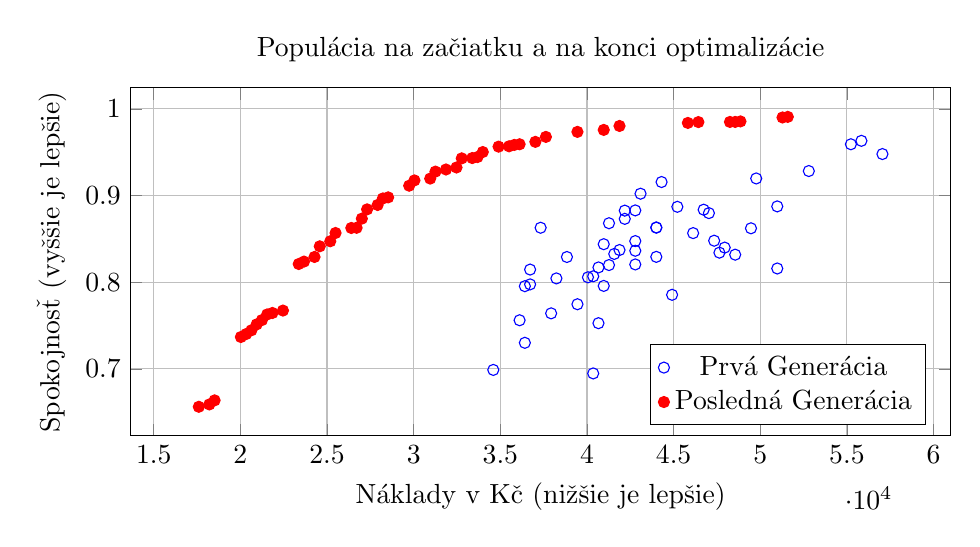
\begin{tikzpicture}
    \begin{axis}[
      xlabel={Náklady v Kč (nižšie je lepšie)},
      ylabel={Spokojnosť (vyššie je lepšie)},
      title={Populácia na začiatku a na konci optimalizácie},
      grid=major,
      legend pos=south east,
      width=12cm,
      height=6cm,
      scatter/classes={
          dominated={mark=o,draw=blue},
          pareto={mark=*,draw=red,fill=red}
      }
    ]
    \addplot[
      scatter,
      only marks,
      scatter src=explicit symbolic
    ]
    table[meta=label] {
      x y label
      34593.6192 0.698766814270199 dominated
      36110.8832 0.7560682593856592 dominated
      36414.335999999996 0.7300462923996281 dominated
      36414.335999999996 0.7953992297817675 dominated
      36717.788799999995 0.8145726857336179 dominated
      36717.788799999995 0.7974700146690784 dominated
      37324.6944 0.8628327143967477 dominated
      37931.6 0.7640401922236763 dominated
      38235.0528 0.8043758906865585 dominated
      38841.958399999996 0.8290733914209067 dominated
      39448.863999999994 0.7745494084899076 dominated
      40055.76959999999 0.8056625705745529 dominated
      40359.2224 0.6947178444331448 dominated
      40359.2224 0.8067975544648183 dominated
      40662.6752 0.8170223752151435 dominated
      40662.6752 0.7526894033690112 dominated
      40966.128 0.7957035301990926 dominated
      40966.128 0.843842264914051 dominated
      41269.580799999996 0.8197795038837332 dominated
      41269.580799999996 0.8680407209612772 dominated
      41573.0336 0.8326062494590158 dominated
      41876.486399999994 0.8371112229491665 dominated
      42179.93919999999 0.8825829363360709 dominated
      42179.93919999999 0.8730773109243625 dominated
      42786.8448 0.847443283201624 dominated
      42786.8448 0.8828430873621682 dominated
      42786.8448 0.8204861227922611 dominated
      42786.8448 0.8362688591286608 dominated
      43090.2976 0.9021138073898618 dominated
      44000.655999999995 0.8631854265897849 dominated
      44000.655999999995 0.8628972991279271 dominated
      44000.655999999995 0.8292353951889984 dominated
      44304.108799999995 0.9155924905270366 dominated
      44911.0144 0.7854295932795443 dominated
      45214.46719999999 0.8869831832852022 dominated
      46124.8256 0.8566406120073122 dominated
      46731.73119999999 0.8836561866125701 dominated
      47035.183999999994 0.8797202797202752 dominated
      47338.6368 0.847873684210521 dominated
      47642.08959999999 0.8340823970037414 dominated
      47945.5424 0.8399150495544213 dominated
      48552.448 0.8317564802182806 dominated
      49462.806399999994 0.8621990315578529 dominated
      49766.25919999999 0.9197099019032373 dominated
      50980.0704 0.8158174027686208 dominated
      50980.0704 0.8874712835025756 dominated
      52800.78719999999 0.9282750998894747 dominated
      55228.40959999999 0.9591714575583303 dominated
      55835.31519999998 0.9631262798634764 dominated
      57049.126399999994 0.947870934959343 dominated
      17600.2624 0.6562155059132695 pareto
      18207.167999999998 0.6589360197949811 pareto
      18510.620799999997 0.6636070458329676 pareto
      20027.884799999996 0.7367264857065519 pareto
      20331.3376 0.7401511514181519 pareto
      20634.790399999998 0.7444830408293153 pareto
      20938.243199999997 0.751307508199624 pareto
      21241.696 0.7562538892345931 pareto
      21545.1488 0.7627662565905033 pareto
      21848.601599999995 0.7644937216136719 pareto
      22455.5072 0.767252314021248 pareto
      23365.865599999994 0.8209870865027319 pareto
      23669.3184 0.8237714587551634 pareto
      24276.224 0.8291082858395329 pareto
      24579.676799999997 0.8413978682509076 pareto
      25186.5824 0.8472269938650214 pareto
      25490.0352 0.8567756029360242 pareto
      26400.393599999996 0.8625608061153471 pareto
      26703.846399999995 0.8627581463330646 pareto
      27007.299199999998 0.8733551273227685 pareto
      27310.752 0.8840321882841456 pareto
      27917.65759999999 0.8890859980831128 pareto
      28221.1104 0.8966087719298096 pareto
      28524.563199999997 0.8978779095300723 pareto
      29738.3744 0.9113484622798445 pareto
      30041.827199999996 0.9174568096114935 pareto
      30952.185599999997 0.9195637058925635 pareto
      31255.6384 0.9275939719383215 pareto
      31862.543999999998 0.930055712693909 pareto
      32469.449599999996 0.9323767361110995 pareto
      32772.9024 0.9428970088078726 pareto
      33379.808 0.9432454753118849 pareto
      33683.2608 0.9444301932576343 pareto
      33986.7136 0.9501810934927507 pareto
      34897.072 0.9564164691422928 pareto
      35503.9776 0.9568245614034963 pareto
      35807.4304 0.9584162615996357 pareto
      36110.8832 0.9591693796744257 pareto
      37021.241599999994 0.9619377043538 pareto
      37628.14719999999 0.9676506396118112 pareto
      39448.863999999994 0.9734642765245602 pareto
      40966.128 0.9757380254154341 pareto
      41876.486399999994 0.9802846167277695 pareto
      45821.3728 0.9837892008639219 pareto
      46428.278399999996 0.9847617435463304 pareto
      48248.99519999999 0.9849325852106111 pareto
      48552.448 0.9849570468656866 pareto
      48855.900799999996 0.9855566716892594 pareto
      51283.52319999998 0.990090885925414 pareto
      51586.975999999995 0.9907816482582757 pareto
    };
    \legend{Prvá Generácia, Posledná Generácia}
    \end{axis}
  \end{tikzpicture}
  \caption{Populácia na začiatku a na konci optimalizácie}
\end{figure}

Na obrázku~\ref{fig:population_start_end} je vidieť priaznivé výsledky optimalizácie.
Algoritmus NSGA-II sa po 100 generáciach priblížil k optimálnemu frontu riešení.
Oproti prvej generácii sa značne znížili náklady a zvýšila spokojnosť cestujúcich.
Tento výsledok ukazuje, že genetický algoritmus dokáže efektívne nájsť kompromis medzi protichodnými cieľmi, ako sú náklady a spokojnosť.
Použitie NSGA-II umožnilo zachovať diverzitu riešení, čo poskytuje používateľovi možnosť výberu najvhodnejšieho časového rozpisu podľa jeho preferencií.

\chapter{Experimenty}\label{experimenty}

V tejto kapitole sú podrobne popísané experimentálne scenáre, ktoré boli navrhnuté na posúdenie výkonnosti optimalizačného algoritmu aplikovaného na plánovanie liniek MHD.
Cieľom bolo preskúmať reakcie algoritmu na zmeny v parametroch ako sú dĺžka trasy, dĺžka vozidla a počet zastávok.

Každý experiment bol vykonaný s rovnakými parametrami pre genetický algoritmus, aby sa zabezpečila konzistentnosť výsledkov:
\begin{itemize}
  \item \textbf{Počet jedincov v populácii} --- 50 pre krátku trasu, 10 pre dlhú trasu \footnote{Tento počet bol znížený z dôvodu dlhej doby výpočtu.}
  \item \textbf{Počet generácií} --- 100
  \item \textbf{Pravdepodobnosť mutácie} --- 5\%
  \item \textbf{Maximálny počet spojov za hodinu} --- 15
\end{itemize}
Ostatné parametre sú špecifické pre jednotlivé experimenty a sú uvedené v tabuľkách v príslušných sekciách.

Parametre zariadenia, na ktorom boli experimenty vykonané, sú:
\begin{itemize}
  \item \textbf{Operačný systém} --- Windows 11 Pro 64-bit
  \item \textbf{Procesor} --- Intel Core i7--9750H CPU @ 2.60GHz
  \item \textbf{RAM} --- 16 GB DDR4
\end{itemize}

Všetky experimenty boli vykonané na rovnakom zariadení, aby sa zabezpečila konzistentnosť výsledkov
a v rovnakom čase, aby sa minimalizoval vplyv vonkajších faktorov.
Každý experiment trval približne od 45 minút do 1.5 hodiny v závislosti od dĺžky trasy a počtu zastávok.

\newpage
\section{Experiment s krátkou trasou a krátkym vozidlom}
Cieľom tohto experimentu je zistiť, ako sa algoritmus vyrovnáva s krátkou trasou a krátkym vozidlom.
Ako referencia bola zvolená linka 46 v Brne, ktorej trasa pozostáva z 11 zastávok.
Parametry experimentu sú uvedené v tabuľke~\ref{tab:shortDshortVin}.

\begin{table}[h]
  \centering
  \begin{tabular}{|l|c|}
    \hline
    \textbf{Vstup} & \textbf{Hodnota} \\ \hline
    Kapacita vozidla & 80 \\ \hline
    Miest na sedenie & 30 \\ \hline
    Celkové náklady & 92,82 Kč/100 miesto-km \\ \hline
    Dĺžka trasy & 3,8 km \\ \hline
  \end{tabular}
  \caption{Parametre vozidla a trasy}
  \label{tab:shortDshortVin}
\end{table}

Ako je vidieť v tabuľke~\ref{tab:shortDshortVout}, optimalizácia prebehla úspešne.
Algoritmus bol schopný vygenerovať rozpis, pri ktorom je spokojnosť cestujúcich 94\% a počet neobslúžených cestujúcich je 0.
Vozidlá sú v priemere zaplnené do jednej tretiny, pretože ich je až 115, to je o 3 vozidlá menej ako je aktuálny rozpis linky 46.
Z toho vyplíva, že musia byť menšie aj celkové prevádzkové náklady linky 46.

\begin{table}[h]
  \centering
  \begin{tabular}{|l|c|}
    \hline
      \textbf{Výstup} & \textbf{Hodnota} \\ \hline
      Počet príchodov cestujúcich & 11603 \\ \hline
      Počet prevezených cestujúcich & 11603 \\ \hline
      Počet neobslúžených cestujúcich & 0 (0,0\,\%) \\ \hline
      Celkový čas strávený čakaním & 54625 min \\ \hline
      Priemerný čas strávený čakaním & 5 min \\ \hline
      Celkové náklady & 32450 Kč \\ \hline
      Priemerná spokojnosť cestujúcich & 94,0\,\% \\ \hline
      Celkový počet vozidiel & 115 \\ \hline
      Priemerná naplnenosť vozidiel & 25 (31,02\,\%) \\ \hline
  \end{tabular}
  \caption{Výstupy simulácie}
  \label{tab:shortDshortVout}
\end{table}

Celý rozpis zastávok, časový rozpis a grafy podrobnejšie popisujúce tento experiment sú uvedené v prílohe~\ref{shortDshortV}.

\newpage

\section{Experiment s krátkou trasou a dlhým vozidlom}
Cieľom tohto experimentu je zistiť, ako sa algoritmus vyrovnáva s krátkou trasou a dlhým vozidlom.
Ako referencia bola zvolená linka 46 v Brne, ktorej trasa pozostáva z 11 zastávok.
Parametry experimentu sú uvedené v tabuľke~\ref{tab:shortDlongVin}.

\begin{table}[h]
  \centering
  \begin{tabular}{|l|c|}
    \hline
    \textbf{Vstup} & \textbf{Hodnota} \\ \hline
    Kapacita vozidla & 160 \\ \hline
    Počet miest na sedenie & 60 \\ \hline
    Celkové náklady & 92,82 Kč/100 miesto-km \\ \hline
    Dĺžka trasy & 3,8 km \\ \hline
  \end{tabular}
  \caption{Parametre vozidla a trasy}
  \label{tab:shortDlongVin}
\end{table}

V tabuľke~\ref{tab:shortDlongVout} sú vidieť výsledky optimalizácie rovnakej linky ako v predošlom experimente, avšak s vozidlom s vyššou kapacitou.
Navýšenie kapacity vozidla má vplyv na:
\begin{itemize}
  \item Priemerná čakacia doba sa zvýšila o 2 minúty
  \item Spokojnosť cestujúcich sa zvýšila o 4,54\%
  \item Počet vozidiel sa znížil o 43 kusov
  \item Priemerná naplnenosť vozidiel sa znížila o 6,42\%
  \item Celkové náklady sa zvýšili o 8183 Kč
\end{itemize}

\begin{table}[h]
  \centering
  \begin{tabular}{|l|c|}
    \hline
      \textbf{Výstup} & \textbf{Hodnota} \\ \hline
      Počet príchodov cestujúcich & 11528 \\ \hline
      Počet prevezených cestujúcich & 11528 \\ \hline
      Počet neobslúžených cestujúcich & 0 (0,0\,\%) \\ \hline
      Celkový čas strávený čakaním & 86013 min \\ \hline
      Priemerný čas strávený čakaním & 7 min \\ \hline
      Celkové náklady & 40633 Kč \\ \hline
      Priemerná spokojnosť cestujúcich & 98,54\,\% \\ \hline
      Celkový počet vozidiel & 72 \\ \hline
      Priemerná naplnenosť vozidiel & 39 (24,6\,\%) \\ \hline
  \end{tabular}
  \caption{Výstupy simulácie}
  \label{tab:shortDlongVout}
\end{table}

Celý rozpis zastávok, časový rozpis a grafy podrobnejšie popisujúce tento experiment sú uvedené v prílohe~\ref{shortDlongV}.

\newpage

\section{Experiment s dlhou trasou a krátkym vozidlom}
Cieľom tohto experimentu je zistiť, ako sa algoritmus vyrovnáva s dlhou trasou a krátkym vozidlom.
Ako referencia bola zvolená okružná linka 84 v Brne, ktorej trasa pozostáva zo 44 zastávok.
Parametry experimentu sú uvedené v tabuľke~\ref{tab:longDshortVin}.

\begin{table}[h]
  \centering
  \begin{tabular}{|l|c|}
    \hline
    \textbf{Vstup} & \textbf{Hodnota} \\ \hline
    Kapacita vozidla & 80 \\ \hline
    Počet miest na sedenie & 30 \\ \hline
    Celkové náklady & 92,82 Kč/100 miesto-km \\ \hline
    Dĺžka trasy & 23,0 km \\ \hline
  \end{tabular}
  \caption{Parametre vozidla a trasy}
  \label{tab:longDshortVin}
\end{table}

Z tabuľky~\ref{tab:longDshortVout} je vidieť, že algoritmus bol schopný vygenerovať rozpis, pri ktorom je spokojnosť cestujúcich viac ako 98\%.
Priemerná čakacia doba, počet vozidiel a priemerná naplnenosť vozidiel sú veľmi podobné ako v prípade krátkej trasy.
Oproti nej však vzrástol počet cestujúcich a teda aj celkový čas strávený čakaním.
Taktiež sa zvýšili celkové náklady na prevádzku.

\begin{table}[h]
  \centering
  \begin{tabular}{|l|c|}
    \hline
      \textbf{Výstup} & \textbf{Hodnota} \\ \hline
        Počet príchodov cestujúcich & 49041 \\ \hline
        Počet prevezených cestujúcich & 49041 \\ \hline
        Počet neobslúžených cestujúcich & 0 (0,0\,\%) \\ \hline
        Celkový čas strávený čakaním & 253052 min \\ \hline
        Priemerný čas strávený čakaním & 5 min \\ \hline
        Celkové náklady & 189576 Kč \\ \hline
        Priemerná spokojnosť cestujúcich & 98,1\,\% \\ \hline
        Celkový počet vozidiel & 111 \\ \hline
        Priemerná naplnenosť vozidiel & 22 (27,67\,\%) \\ \hline
  \end{tabular}
  \caption{Výstupy simulácie}
  \label{tab:longDshortVout}
\end{table}

Celý rozpis zastávok, časový rozpis a grafy podrobnejšie popisujúce tento experiment sú uvedené v prílohe~\ref{longDshortV}.

\newpage
\section{Experiment s dlhou trasou a dlhým vozidlom}
Cieľom tohto experimentu je zistiť, ako sa algoritmus vyrovnáva s dlhou trasou a dlhým vozidlom.
Ako referencia bola zvolená okružná linka 84 v Brne, ktorej trasa pozostáva zo 44 zastávok.
Parametry experimentu sú uvedené v tabuľke~\ref{tab:longDlongVin}.

\begin{table}[h]
  \centering
  \begin{tabular}{|l|c|}
    \hline
    \textbf{Vstup} & \textbf{Hodnota} \\ \hline
    Kapacita vozidla & 160 \\ \hline
    Počet miest na sedenie & 60 \\ \hline
    Celkové náklady & 92,82 Kč/100 miesto-km \\ \hline
    Dĺžka trasy & 23,0 km \\ \hline
  \end{tabular}
  \caption{Parametre vozidla a trasy}
  \label{tab:longDlongVin}
\end{table}

Výstupy experimentu je možné vidieť v tabuľke~\ref{tab:longDlongVout}.
Oproti experimentu s dlhou cestou ale krátkym vozidlom sa zmenili následovné parametre:
\begin{itemize}
  \item Priemerná čakacia doba sa zvýšila o 2 minúty
  \item Spokojnosť cestiujúcich sa zvýšila o 1,88\%
  \item Počet vozidiel sa znížil o 29 kusov
  \item Priemerná naplnenosť vozidiel sa znížila o 9,04\%
  \item Celkové náklady sa zvýšili o 90518 Kč
\end{itemize}

\begin{table}[h]
  \centering
  \begin{tabular}{|l|c|}
    \hline
      \textbf{Výstup} & \textbf{Hodnota} \\ \hline
        Počet príchodov cestujúcich & 48358 \\ \hline
          Počet prevezených cestujúcich & 48358 \\ \hline
          Počet neobslúžených cestujúcich & 0 (0,0\,\%) \\ \hline
          Celkový čas strávený čakaním & 314379 min \\ \hline
          Priemerný čas strávený čakaním & 7 min \\ \hline
          Celkové náklady & 280094 Kč \\ \hline
          Priemerná spokojnosť cestujúcich & 99,98\,\% \\ \hline
          Celkový počet vozidiel & 82 \\ \hline
          Priemerná naplnenosť vozidiel & 30 (18,63\,\%) \\ \hline
  \end{tabular}
  \caption{Výstupy simulácie}
  \label{tab:longDlongVout}
\end{table}

Celý rozpis zastávok, časový rozpis a grafy podrobnejšie popisujúce tento experiment sú uvedené v prílohe~\ref{longDlongV}.

\chapter{Nástroj na analýzu a optimalizáciu časových rozpisov}\label{nastroj}

Poslednou časťou tejto práce je implementácia nástroja na analýzu a optimalizáciu časových rozpisov.
Tento nástroj slúži ako rozhranie medzi požívateľom a optimalizačným algoritmom.
Nástroj bude mať dve hlavné funkcie:
\begin{itemize}
  \item \textbf{Analýza časového rozpisu} --- nástroj prevezme existujúci časový rozpis a vykoná analýzu jeho kvality. Na to poslúži spustenie simulácie, zber štatistík a ich vizualizácia.
  \item \textbf{Optimalizácia časového rozpisu} --- nástroj vygeneruje nové časové rozpisy na základe vstupných parametrov a požiadaviek používateľa. Na to poslúži optimalizačný algoritmus NSGA-II.
\end{itemize}

Používateľské rozhranie by malo byť intuitívne a jednoduché.
Hlavným cieľom tejto práce je optimalizácia, preto je kladený väčší dôraz na ňu ako na samotné používateľské rozhranie.
Toto rozhranie je pre používanie optimalizačného algoritmu nevyhnutné, bez ohľadu na jeho jednoduchosť, nesmie byť jeho vývoj zanedbaný.

\section{Návrh používateľského rozhrania}\label{nastroj_uzivatelske_rozhranie}

Prvý krok pri tvorbe používateľských rozhraní je jeho návrh.
Je dôležité si premyslieť funkcionalitu akú bude rozhranie poskytovať.
Tento nástroj by mal vedieť analyzovať nainportované časové rozpisy, vizualizovať výsledky simulácie, prezentovať ich formou grafov a štatistík a optimalizovať časové rozpisy.
Výpočet optimalizácie pomocou genetického algoritmu je časovo náročný úkon a preto je nutné používateľa informovať o jeho priebehu formou zobrazenia aktuálnej generácie.
Po dokončení optimalizácie bude mať používateľ možnosť vybrať si rozpis, ktorý najviac zodpovedá jeho potrebám a uložiť si ho.
Používateľské rozhranie by malo umožniť aj analýzu už uložených rozpisov, prípadne export jednotlivých analýz do napríklad textového súboru alebo PDF.

Všetky uvedené funkcie budú rozdelené medzi dve stránky, stránku pre analýzu a stránku pre optimalizáciu.
Na prepínanie medzi stránkami bude slúžiť jednoduché menu v hornej časti okna.
Na ich návrh boli použité wireframy.

\newpage
\subsection*{Stránka pre analýzu časového rozpisu}
Na stránke analýzy časového rozpisu bude možné:
\begin{itemize}
  \item naimportovať informácie o zastávkach
  \item naimportovať informácie o časovom rozpise
  \item vybrať uložený časový rozpis
  \item zadať parametre pre simuláciu
  \item resetovať stránku (vyprázdniť vstupy)
  \item spustiť simuláciu
  \item zobraziť výsledky analýzy, vrátane grafov a štatistík
  \item uložiť výsledky analýzy
\end{itemize}

\begin{figure}[h]\label{fig:wireframe_analyze}
  \centering
  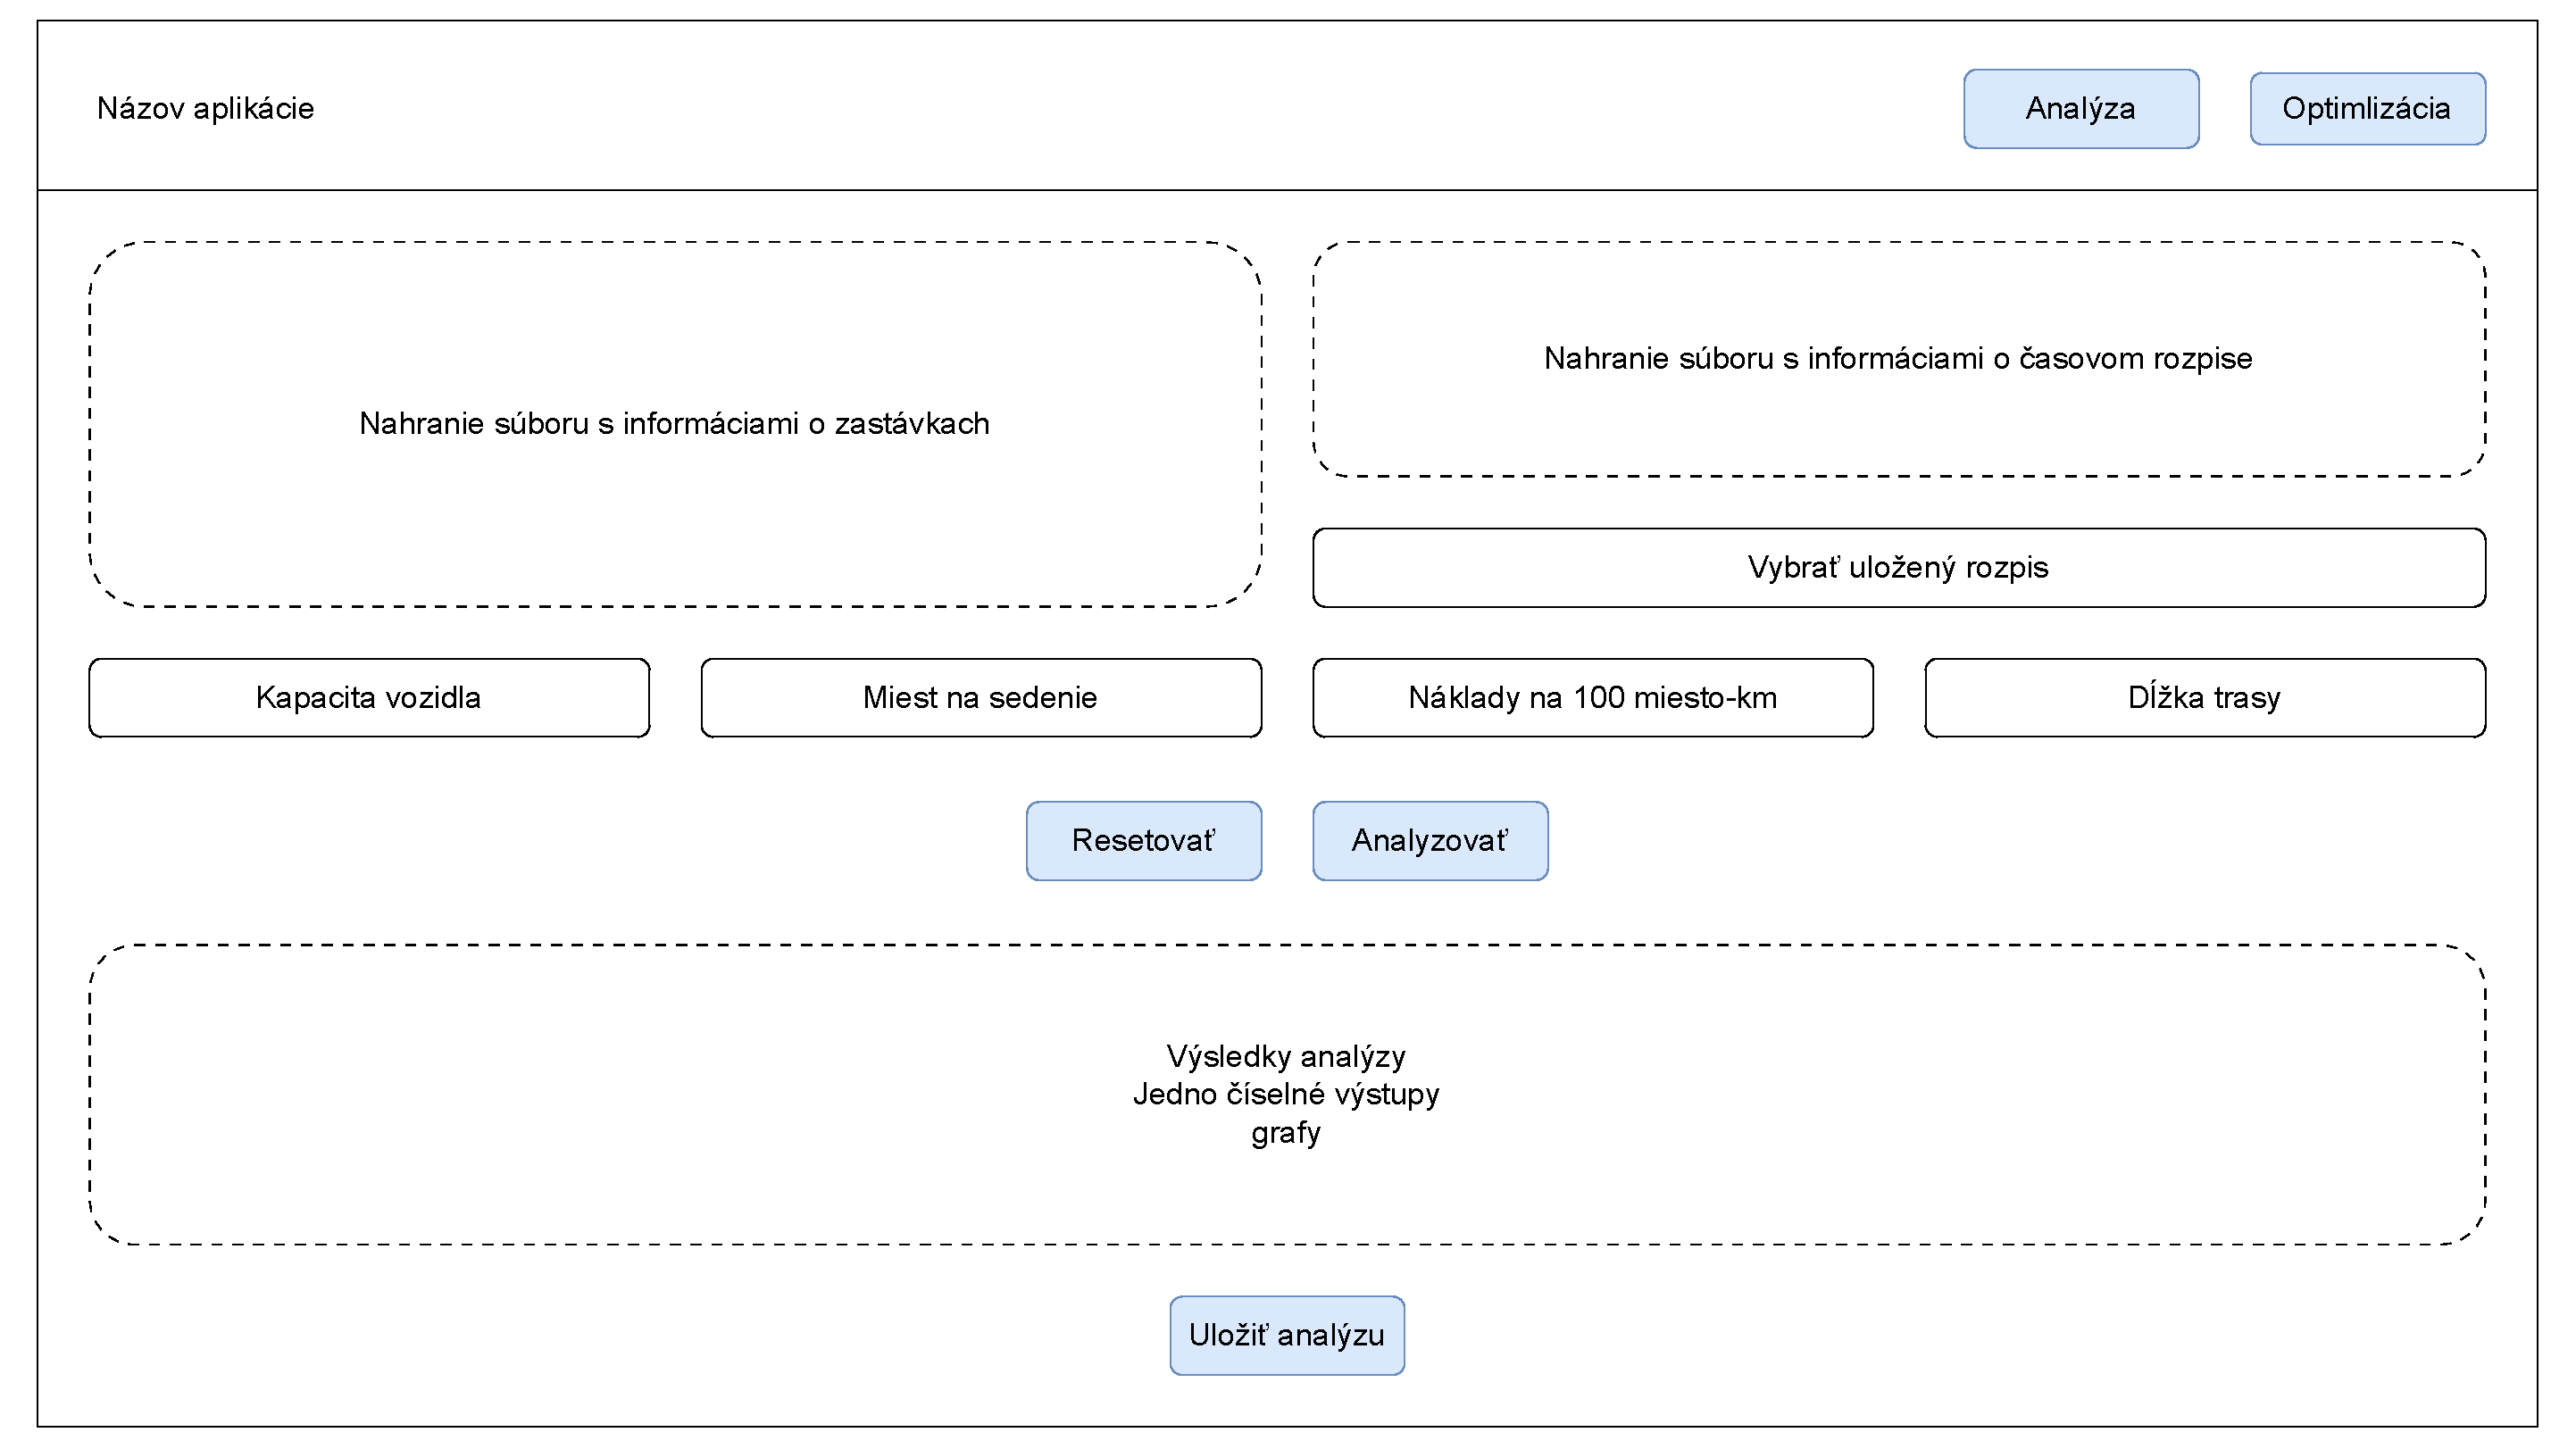
\includegraphics[width=\textwidth]{wireframe_analyze.pdf}
  \caption{Wireframe pre analýzu časového rozpisu}
\end{figure}

Na obrázku~\ref{fig:wireframe_analyze} je znázornený wireframe pre túto stránku.
Funkcie spomenuté vyššie sú usporiadané rovnako ako jednotlivé elementy stránky.
Na import informácií o zastávke a nového časového ropisu bude slúžiť vyberač súborov.
Importný súbor bude vo formáte TXT.
Uživateľské rozhranie by malo obsahovať nápovedu, ktorá používateľovi poskytne vzor formátu vsupných súborov.

\noindent Formát potrebný na import informácií o zastávkach:

\noindent \texttt{Lesná, Haškova:0:[(5, 60), (6, 90), \ldots , (21, 40), (22, 30)]:0 \newline
  Brechtova:1:[(5, 60), (6, 90), \ldots , (21, 40), (22, 30)]:0.1 \newline
  Blažkova:2:[(5, 60), (6, 90), \ldots , (21, 40), (22, 30)]:0.1 \newline
  \ldots
}

\noindent Formát potrebný na import informácií o časovom rozpise:

\noindent \texttt{04: \newline
  05:01,11,21,31,41,51 \newline
  06:01,08,14,21,28,34,41,48,54 \newline
  07:01,08,14,21,28,34,41,48,54 \newline
  08:01,08,18,28,38,48,58 \newline
  09:08,18,28,38,48,58 \newline
  \ldots
}

Výber uloženého rozpisu môže byť realizovaný formou rozbaľovacej ponuky.
Rozpisy v tejto ponuke by mali byť pomenované, aby bol výber prehľadný.
Vstupné parametre \texttt{Kapacita vozidla}, \texttt{Miest na sedenie}, \texttt{Náklady na 100 miesto-km} a \texttt{Dľžka trasy} budú realizované jednoduchými textovými vstupmi, s obmedzením len na numerické znaky, prípadne číslenými obmedzeniami potrebnými pre dané parametre.
Tlačítko \texttt{Resetovať} vymaže všetky vstupy aj výstupy analýzy.
Tlačítko \texttt{Analyzovať} spustí simuláciu časového rozpisu a zobrazí výsledky analýzy.
Medzi tieto výsledky budú patriť agregované hodnoty:
\begin{itemize}
  \item Počet príchodov cestujúcich
  \item Počet prevezených cestujúcich
  \item Počet neobslúžených cestujúcich
  \item Celkový čas strávený čakaním
  \item Priemerný čas strávený čakaním
  \item Celkové náklady
  \item Priemerná spokojnosť cestujúcich
  \item Celkový počet vozidiel
  \item Priemerná naplnenosť vozidiel
\end{itemize}
Taktiež budú na stránke zobrazené grafy s hodnotami rôznych štatistík za hodinu, aby boli vidieť zmeny v priebehu dňa, konkrétne:
\begin{itemize}
  \item Cestujúci prichádzajúci za hodinu
  \item Priemerný čas strávený čakaním za hodinu
  \item Počet neobslúžených cestujúcich za hodinu
\end{itemize}
Posledným grafom bude:
\begin{itemize}
  \item Priemerná naplnenosť vozidiel na linke
\end{itemize}
Po stlačení tlačítka \texttt{Uložiť analýzu} sa otvorí vyberač súborov, aby si používateľ mohol z adresárovej štruktúry vybrať kam sa vygenerovaného analýza uloží.
Analýza sa bude ukladať vo formáte TXT.

\newpage
\subsection*{Stránka pre optimalizáciu časového rozpisu}
Na stránke optimalizácie časového rozpisu bude možné:
\begin{itemize}
  \item naimportovať informácie o zastávkach
  \item zadať parametre pre optimalizáciu
  \item Resetovať stránku
  \item spustiť optimalizáciu
  \item zobraziť priebežne dosiahnuté cieľe aktuálne spracovanej generácie
  \item vybrať rozpis z generácie
  \item uložiť vybraný rozpis
\end{itemize}

\begin{figure}[h]\label{fig:wireframe_optimize}
  \centering
  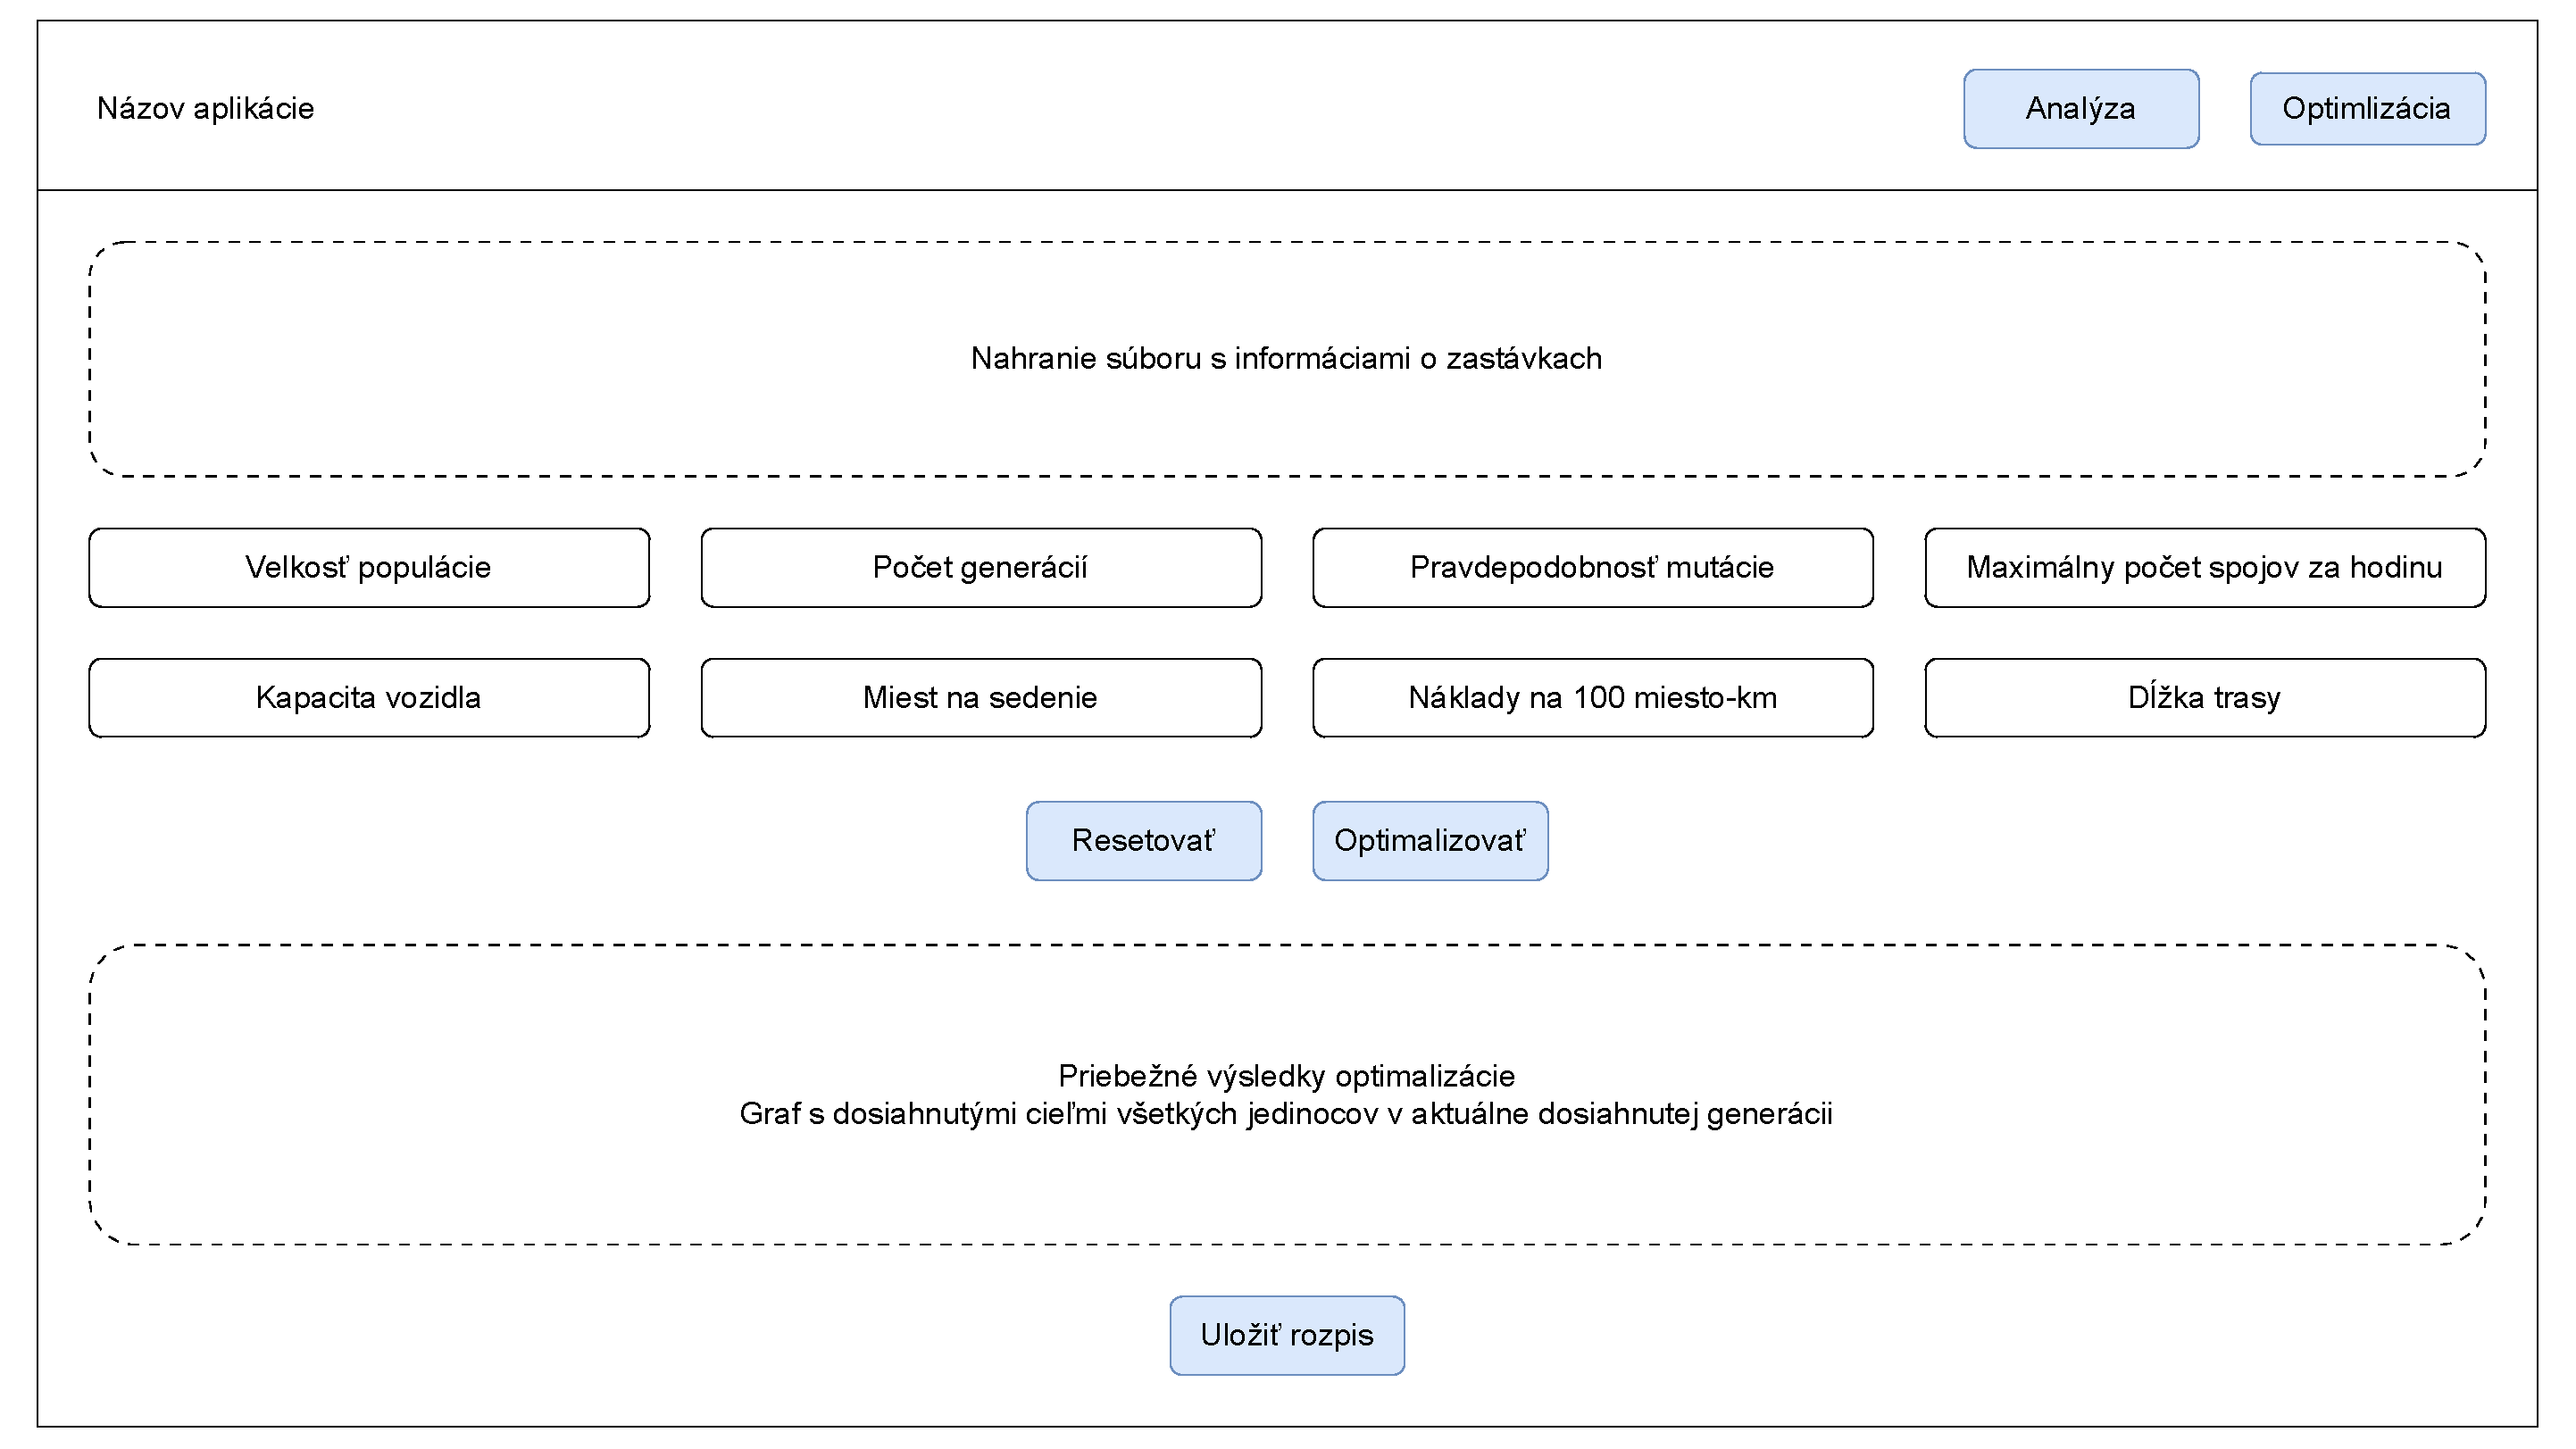
\includegraphics[width=\textwidth]{wireframe_optimize.pdf}
  \caption{Wireframe pre optimalizáciu časového rozpisu}
\end{figure}

Na obrázku~\ref{fig:wireframe_optimize} je znázornený wireframe pre túto stránku.
Pre nahranie informácií o zastávke bude slúžiť rovnaký vyberač súborov ako na stránke analýzy.
Vyberač pre časový rozpis v tomto prípade nie je potrebný, pretože z pohľadu optimalizácie je časový rozpis výstupom a nie vstupom.
Číselné vstupné parametre pre simuláciu sú rovnaké ako na stránke analýzy, ale pre genetický algoritmus je navyše potrebné zadať štyri nové a to \texttt{Velkosť populácie}, \texttt{Počet generácií}, \texttt{Pravdepodobnosť mutácie} a \texttt{Maximálny počet spojov za hodinu}.
Tlačítko \texttt{Resetovať} vymaže všetky vstupy aj výstupy optimalizácie.
Tlačítko \texttt{Optimalizovať} spustí optimalizáciu časového rozpisu.
Používateľ by mal počas optimalizácie byť schopný vidieť:
\begin{itemize}
  \item Ktorú generáciu algoritmus aktuálne spracováva
  \item Koľko generácií bude algoritmus spracovávať
  \item Kedy optimalizácia začala
  \item Kedy optimalizácia skončila (ak už skončila)
  \item Ako dlho optimalizácia trvala (ak už skončila)
  \item Graf s priebežnými dosiahnutými cieľmi jednotlivých jedincov v aktuálne dosiahnutej generácii
\end{itemize}
Po dokončení optimalizácie by mal byť používateľ schopný prezrieť si všetky rozpisy v poslednej generácii.
To bude zabezpečené posuvným tiahlom a zobrazením aktuálne vybraného rozpisu.
Tiahlo bude mať toľko krokov, koľko je rozpisov v generácii.
Vyplnením textového vstupu pre názov rozpisu a stlačením tlačítka \texttt{Uložiť rozpis} sa rozpis uloží.
Nepomenovaný rozpis sa pri uložení automaticky pomenuje časom a dátumom jeho vytvorenia %TODO dopisat format

\section{Implementácia nástroja}\label{nastroj_implementacia}

Po návrhu následuje implementácia.
Prvým krokom implementácie je výber vhodných technológií a druhým je návrh architektúry aplikácie.

\subsection*{Použité technológie}
Ako programovací jazyk bol zvolený \texttt{Python} a to preto, lebo je veľmi verzatilný.
Ďalšou možnosťou by bolo naprogramovať optimalizačný algoritmus v jazyku \texttt{C} alebo \texttt{C++}, ktoré sú rýchlejšie.

\texttt{Python} bol však vybraný vďaka jednoduchému použitiu a možnostiam naprogramovania ako backendu, tak aj frontendu (na programovanie frontendu bol využitý framework \texttt{Reflex}~\cite{reflex_docs}).

Vďaka tomuto frameworku je možné písať webové komponenty a celé stránky priamo v jazyku \texttt{Python}.
Každý komponent je písaný formou funkcie, ktorá vracia jeho obsah.
Tým sa dajú komponenty zhlukovať do väčších komponentov alebo stránok.
Vstupy komponentov sa dajú predávať ako parametre jeho funkcie alebo môže komponent pracovať s premennými, ktoré sú súčasťou triedy \texttt{State}.
\texttt{State} je trieda, ktorá počas behu aplikácie uchováva jej stav.
K premenným tohto stavu sa dá jednoducho pristupovať, čítať ich hodnoty aj prepisovať ich.
Takýchto tried môže byť v aplikácii viacej a jeden komponent môže pracovať s premennými viacerých stavov.
Stav okrem premenných obsahuje aj metódy, ktoré sa volajú pri danej udalosti.
Medzi udalosti patrí napríklad stlačenie konkrétneho tlačítka alebo zmena hodnoty v jednom z textových vstupov.
V týchto metódach sa môže pristupovať aj k premenným iného stavu.               

Informácie o použítí tohoto frameworku boli čerpané z jeho oficiálnej dokumentácie~\cite{reflex_docs}.

Takáto verzatilita jazyka a frameworku bola pri programovaní tohto nástroja veľmi vítaná,
treba však dávať pozor na prehladnosť a previazanosť kódu aby sa v budúcnosti dal ľahko rozširovať.
Je potrebné zvoliť si dobrú architektúru, rozčlenenie aplikácie na moduly a tie na jednotlivé webové komponenty alebo backendové skripty, pretože tieto technológie umožňujú veľkú variabilitu písania zdrojového kódu aplikácie.

\subsection*{Architektúra aplikácie}
Aplikácia sa volá SPROUT, čo znamená \textit{Smart Performance and Resource Optimization for Urban Transport}, po slovensky inteligentná optimalizácia výkonu a zdrojov verejnej dopravy.
Touto skratkou je označený aj hlavný adresár, ktorý obsahuje všetky zdrojové kódy aplikácie.
V ňom sa nachádzajú adresáre \texttt{backend}, v ktorom sú skripty obsahujúce logiku, simulačný model, kalendár udalostí, genetický algoritmus a podobné, \texttt{components}, ktorý obsahuje webové komponenty a \texttt{pages}, kde sú uložené zdrojové kódy jednotlivých stránok aplikácie.
Ďalej sa tu nachádza \texttt{sprout.py}, súbor, ktorý obsahuje koreňový element aplikácie a smerovanie medzi jednotlivými stránkami.
Posledným súborom v tomto adresári je \texttt{\_\_init\_\_.py}, ktorý slúži na inicializáciu adresára ako \texttt{Python} modulu.
Tento inicializačný súbor sa nachádza aj vo všetkých ostatných adresároch.

\dirtree{%
  .1 sprout.
  .2 backend.
  .3 \_\_init\_\_.py.
  .3 EventCalendar.py.
  .3 Genetics.py.
  .3 InputParser.py.
  .3 models.py.
  .3 RandomNumberGenerator.py.
  .3 Simulation.py.
  .3 Statistics.py.
  .2 components.
  .3 \_\_init\_\_.py.
  .3 analyzeLine.py.
  .3 busStopChart.py.
  .3 busStopTable.py.
  .3 constraintInput.py.
  .3 footer.py.
  .3 hourChart.py.
  .3 infoCard.py.
  .3 infoUpload.py.
  .3 layout.py.
  .3 navbar.py.
  .3 numberInput.py.
  .3 optimizeLine.py.
  .3 rozpis.txt.
  .3 timeTable.py.
  .3 zastavky.txt.
  .2 pages.
  .3 \_\_init\_\_.py.
  .3 analyzePage.py.
  .3 homePage.py.
  .3 optimizePage.py.
  .2 \_\_init\_\_.py.
  .2 sprout.py.
}

\newpage

\begin{table}[h]\label{tab:source_codes}
  \centering
  \begin{tabularx}{\textwidth}{|l|X|}
    \hline
    \textbf{Súbor} & \textbf{Obsah} \\ \hline
    Backendové skripty & \\
    EventCalendar.py & trieda kalendára udalostí a udalosti \\
    Genetics.py & trieda genetického algoritmu a jedného jedinca \\
    InputParser.py & trieda s metódami na spracovanie vstupu \\
    models.py &  model zastávky, vozidla a časového rozpisu\\
    RandomNumberGenerator.py & trieda generátora náhodných čísel \\
    Simulation.py & trieda na riadenie simulácie \\
    Statistics.py & trieda na zber a spracovanie štatistík \\ \hline
    Webové komponenty & \\
    analyzeLine.py & analýza časového rozpisu \\
    busStopChart.py & zobrazenie grafu so zastávkami na osi x \\
    busStopTable.py &zobrazenie tabuľky so zastávkami \\
    constraintInput.py & zadanie obmedzení počtu spojov za hodinu \\
    footer.py & pätička webovej aplikácie \\
    hourChart.py & zobrazenie grafu s hodinami na osi x \\
    infoCard.py & zobrazenie jednočíselných štatistík \\
    infoUpload.py & import súboru \\
    layout.py & základné rozloženie stránky \\
    navbar.py & vrchné navigačné menu \\
    numberInput.py & zadanie jednočíselných vstupov \\
    optimizeLine.py & optimalizácia časového rozpisu \\
    rozpis.txt & vzorový príklad informácií o časovom rozpise \\
    timeTable.py & zobrazenie časového rozpisu \\
    zastavky.txt & vzorový príklad informácií o zastávkach \\ \hline
    Stránky aplikácie & \\
    analyzePage.py & stránka pre anaýlzu časového rozpisu \\
    homePage.py & úvodná stránka \\
    optimizePage.py & stránka pre optimalizáciu časového rozpisu \\ \hline
    sprout.py & koreňový komponent a smerovanie \\ \hline
  \end{tabularx}
  \caption{Zdrojové kódy}
\end{table}

V tabuľke~\ref{tab:source_codes} je stručne popísaný obsah jednotlivých súborov zdrojových kódov a ich rozdelenie medzi jednotlivé moduly.
Podrobnejší popis celého zdrojového kódu je dostupný v programovej dokumentácii~\cite{sprout_docs}, ktorá bola vygenerovaná pomocou nástroja \texttt{Sphinx}~\cite{sphinx_doc}.

\subsection*{Inštalácia a spustenie aplikácie}
Postup inštalácie a spustenia aplikácie na lokálnom počítači je nasledovný:
\begin{enumerate}
  \item Nainštalujte si \texttt{Python} vo verzii 3.10.
  \item Nainštalujte si \texttt{pip} vo verzii 24.3.
  \item (Volitelné) v koreňovom adresári projektu vytvorte virtuálne prostredie príkazom \texttt{python -m venv venv}.
  \item Aktivujte virtuálne prostredie príkazom \texttt{venv\textbackslash Scripts\textbackslash activate} na Windowse alebo \texttt{source venv/bin/activate} na Linuxe.
  \item Nainštalujte potrebné knižnice príkazom \texttt{pip install -r requirements.txt}.
  \item Pomocou príkazu \texttt{cd src/sprout} sa presuňte do adresára s aplikáciou.
  \item Spustite aplikáciu príkazom \texttt{reflex run}.
\end{enumerate}

\chapter{Záver}\label{zaver}

Cieľom tejto práce bolo vyvinúť nástroj, ktorý by umožnil zjednodušene optimalizovať mestskú hromadnú dopravu.
Ako cieľ optimalizácie bol vybraný časový rozpis linky MHD.
Optimalizácia bola realizovaná pomocou multi-objektívneho genetického algoritmu NSGA-II.

Táto práca mala splniť následujúce body:
\begin{enumerate}
  \item Preskúmajte problematiku vytvárania siete mestskej hromadnej dopravy, jej modelovania a optimalizácie pre mestá do pol milióna obyvateľov. Na návrh môjho garanta bol simulačný model navrhnutý pomocou DEVS, poznatky o tomto formalizme boli čerpané zo zborníku z konferencie WSC~\cite{tendeloo2018discrete} a príklad, ktorý pomohol k lepšiemu porozumeniu tejto témy je čerpaný z článku~\cite{seo2014devs}. 
  \item Pre mesto veľkosti krajského mesta Českej republiky získajte alebo odhadnite dáta, z ktorých zostavíte model miestnej mestskej hromadnej dopravy. Informácie boli získané priamo z Dopravného podniku mesta Brno, podrobnejší popis je v kapitole~\ref{relevantne_vlastnosti}.
  \item Oboznámte sa s riešeniami, ktoré na optimalizáciu takejto siete používajú metódy umelej inteligencie. Inšpirácia na použitie genetického algoritmu vychádza z vedeckého článku~\cite{tang2021data}, konkrétne ide o multi-objektívny NSGA-II.\@
  \item Vytvorte prostredie, ktoré bude slúžiť na modelovanie a optimalizáciu takejto siete. Bol vytvorený nástroj na analýzu a optimalizáciu časových rozpisov, ktorý je popísaný v kapitole~\ref{nastroj}, na zostrojenie modelu slúžia používateľské vstupy, ktoré nástroj spracuje a sám zostrojí model.
  \item Na vhodne zvolených príkladoch overte fungovanie vášho systému a diskutujte dosiahnuté výsledky. Fungovanie systému bolo otestované v rámci štyroch experimentov a priebežného testovania počas vývoja. Experimenty sú v kapitole~\ref{experimenty}. Výsledky preukázali, že algoritmus je schopný sa prispôsobiť rôznym situáciam.
\end{enumerate}

Aplikáciu by bolo možné rozšíriť napríklad o porovnanie dvoch rozpisov, alebo exportovanie analýzy vo formáte PDF, alebo export optimalizácie, rozšírenie nástroja o verzatilnejšie zadávanie vstupov nakoľko momentálny import údajov o zastávkach a časovom rozpise je možný len vo formáte TXT.
Pri analýze a optimalizácii sa využíva simulačný model, ktorý je možné spraviť podrobnejší, aby sa viac približoval realite a dodal tak ešte kvalitnejšie výsledky.
V rámci optimalizácie by sa mohli niektoré výpočty sparalelizovať tak, aby sa skrátila doba čakania na výsledok.
Bolo by možné rozšíriť optimalizáciu o inteligentné ohodnocovanie rozpisov v poslednej generácii na základe nových používateľských vstupov, aby sa eliminoval ručný výber najvhodnejšieho rozpisu používateľom.
